\chapter{Certifiable Trajectory Optimization via Semidefinite Relaxation}
\label{chapter:certifiable_trajectory_optimization}

This chapter formulates the discrete rigid-body models derived in 
Chapter \ref{chapter:discrete_mechanics_for_rigid_bodies_on_lie_groups} as 
finite-horizon trajectory optimization problems. Section \ref{sec:discrete_motion_planning_of_rigid_body_systems} 
introduces the geometric motion planning 
formulation of \cite{Sangli2025}, which expresses the Lie group variational 
integrators and their kinematic constraints by polynomial equalities and inequalities. 
In general, a nonconvex polynomial optimization problem is relaxed to a convex semidefinite 
program. Therefore, Section \ref{sec:semidefinite_optimization_relaxation} gives an 
overall introduction to semidefinite programming and presents the 
Moment-SOS hierarchy and the exploitation of correlative and term sparsity. 
Finally, Sections \ref{sec:discrete_motion_planning_3d_pendulum} and 
\ref{sec:discrete_motion_planning_acrobot} define the optimization formulation for 
the controlled 3D-pendulum and the Acrobot. The resulting construction follows the sparse 
semidefinite trajectory optimization framework SPOT of \cite{Kang_2026Fast,Kang_2025Global}.
For the Acrobot, the sparse SDP relaxation is embedded in a model predictive control loop. 
Because the prediction-horizon relaxation is not rank one, the extracted predicted trajectory 
is not certified as globally optimal or feasible. Nevertheless, applying the first extracted 
control and simulating the controlled LGVI produces a 
dynamically consistent numerical closed-loop trajectory.

\section{Discrete Motion Planning of Rigid-Body Systems}
\label{sec:discrete_motion_planning_of_rigid_body_systems}

A general robot motion planning problem is modeled as a mechanical system 
consisting of \(n_{\mathrm b}\) rigid links, 
indexed by \(i\in\mathcal B:=\{1,\ldots,n_{\mathrm b}\}\), with $N$ steps starting at $k=0$. 
The robot configuration state \(\bm{Y}_k\) consists of the center-of-mass positions \(\bm{x}_{i,k}\), 
rotations \(\bm{R}_{i,k}\). The relative rotations \(\bm{F}_{i,k}\) are recunstructed from the 
kinematic update \eqref{eq:discrete_lie_group_kinematics}. The control input is denoted 
by \(\bm{U}_{k+1}\), with \(\bm{\lambda}_{k+1}\) being the Lagrange multipliers of the holonomic joint 
constraints. Adapted from the discrete kinodynamic motion planning problem of 
\cite{Sangli2025}, the general multi-body problem is written as
\begin{subequations}
\label{eq:general_motion_optimization}
\begin{align}
\min_{\{\bm{Y}_k\}_{k=0}^{N},\{\bm{U}_k,\bm{\lambda}_k\}_{k=1}^{N}}
&\quad \Psi(\bm{Y}_N)+\sum_{k=0}^{N-1}\psi(\bm{Y}_k,\bm{U}_{k+1},\bm{\lambda}_{k+1})\\
\text{s.t.}\quad
&\mathcal D_i(\bm{Y}_{k+1},\bm{Y}_k,\bm{U}_{k+1},\bm{\lambda}_{k+1})=0, \qquad i\in\mathcal B,\\
&\bm{Y}_k\in\mathcal Y_i, \\
&\mathcal{H}(\bm{Y}_{k+1},\bm{U}_{k+1},\bm{\lambda}_{k+1})\geq0,\\
&\bm{U}_{\min}\leq \bm{U}_{k+1}\leq \bm{U}_{\max},\\
&\bm{Y}_0=\bm{Y}_{\mathrm{init}},\\
&k=0,\ldots,N-1. \nonumber
\end{align}
\end{subequations}
Here, \(\Psi(\cdot)\) denotes the terminal costs and \(\psi(\cdot)\) the running costs. 
The equality constraint set \(\mathcal D_i=0\) represents the forced 
discrete Euler--Lagrange equations of link \(i\) derived in Chapter \ref{chapter:discrete_mechanics_for_rigid_bodies_on_lie_groups}, 
including the set of control inputs $\bm{U}_{k+1}$ and Lagrange multipliers $\bm{\lambda}_{k+1}$. Additionally,
for multi-body systems, the set
\(\mathcal D_i\) contains the holonomic joint constraints \eqref{eq:holonomic_constraints_general}.
The inequalities \(\mathcal{H}\geq0\) describe rotation-step limits, 
geometric constraints such as collision avoidance, and bounds introduced to obtain a compact feasible set \cite{Kang_2026Fast}. 
Control limits are set by \(\bm{U}_{\min}\leq \bm{U}_k\leq \bm{U}_{\max}\) in \eqref{eq:general_motion_optimization}.

The set \(\mathcal Y_i\) enforces the matrix Lie-group structure of the set of states $\bm{Y}_k$. 
Thereby, the multiplicative kinematic update 
\begin{equation}
\bm{R}_{i,k+1}=\bm{R}_{i,k}\bm{F}_{i,k}
\label{eq:general_lie_group_kinematics}
\end{equation}
preserves the corresponding Lie group structure for each link \(i\). 

For rigid-body motion on $SO(3)$, 
the rotation of link \(i\) is given by
\[
\bm{R}_{i,k}=
\begin{bmatrix}
\bm{r}^{1}_{i,k},&\bm{r}^{2}_{i,k},&\bm{r}^{3}_{i,k}
\end{bmatrix}
\in\mathbb R^{3\times3}.
\]
Following \cite{Sangli2025}, 
$\bm{R}_{i,k} \in \mathrm{SO}(3)$ is represented by the 
15 quadratic polynomial equalities
\begin{align}
&\|\bm{r}^{1}_{i,k}\|_2^2-1
=
\|\bm{r}^{2}_{i,k}\|_2^2-1
=
\|\bm{r}^{3}_{i,k}\|_2^2-1
=0,\nonumber\\
&(\bm{r}^{1}_{i,k})^\top \bm{r}^{2}_{i,k}
=
(\bm{r}^{2}_{i,k})^\top \bm{r}^{3}_{i,k}
=
(\bm{r}^{1}_{i,k})^\top \bm{r}^{3}_{i,k}
=0,
\label{eq:so3_polynomial_constraints}\\
&\bm{r}^{1}_{i,k}\times \bm{r}^{2}_{i,k}-\bm{r}^{3}_{i,k}
=
\bm{r}^{2}_{i,k}\times \bm{r}^{3}_{i,k}-\bm{r}^{1}_{i,k}
=
\bm{r}^{3}_{i,k}\times \bm{r}^{1}_{i,k}-\bm{r}^{2}_{i,k}
=\bm{0}_{3\times1}.
\nonumber
\end{align}
The same constraints are imposed on \(\bm{F}_{i,k}\) by replacing
\(\bm{r}^{1}_{i,k},\bm{r}^{2}_{i,k},\bm{r}^{3}_{i,k}\) with its columns
\(\bm{f}^{1}_{i,k},\bm{f}^{2}_{i,k},\bm{f}^{3}_{i,k}\).

For rigid-body motion on $SO(2)$, the standard polynomial parametrization is
\begin{equation}
\bm{R}_{i,k}=
\begin{bmatrix}
c_{i,k}&-s_{i,k}\\
s_{i,k}&c_{i,k}
\end{bmatrix},
\qquad
\bm{F}_{i,k}=
\begin{bmatrix}
a_{i,k}&-b_{i,k}\\
b_{i,k}&a_{i,k}
\end{bmatrix},
\end{equation}
where \(c_{i,k}=\cos\theta_{i,k}\), \(s_{i,k}=\sin\theta_{i,k}\), \(a_{i,k}=\cos\Delta\theta_{i,k}\), and \(b_{i,k}=\sin\Delta\theta_{i,k}\) \cite{Hall2000LieGroups}. 
Applying \eqref{eq:so2_polynomial_constraints} 
to the kinematic update for each link \(i\) in \eqref{eq:general_lie_group_kinematics},
its planar version is given by
\begin{align}
c_{i,k+1}-c_{i,k}a_{i,k}+s_{i,k}b_{i,k}=0,
\qquad
s_{i,k+1}-s_{i,k}a_{i,k}-c_{i,k}b_{i,k}=0,
\end{align}
for planar motion. In contrast to \eqref{eq:so3_polynomial_constraints}, the planar rotation matrices
\(\bm{R}_{i,k},\bm{F}_{i,k} \in \mathrm{SO}(2)\) are imposed by the two quadratic polynomial equalities
\begin{align}\label{eq:so2_polynomial_constraints}
c_{i,k}^2+s_{i,k}^2=1,
\qquad
a_{i,k}^2+b_{i,k}^2=1, 
\end{align}
\cite{Sangli2025}.

The matrix in \eqref{eq:so2_polynomial_constraints} describes a rotation in the \(xy\)-plane and therefore about the \(z\)-axis. In general, rotations about a fixed axis are
\begin{equation}
\bm{R}_x=
\begin{bmatrix}
1&0&0\\
0&c&-s\\
0&s&c
\end{bmatrix},
\qquad
\bm{R}_y=
\begin{bmatrix}
c&0&s\\
0&1&0\\
-s&0&c
\end{bmatrix},
\qquad
\bm{R}_z=
\begin{bmatrix}
c&-s&0\\
s&c&0\\
0&0&1
\end{bmatrix},
\label{eq:axis_rotations}
\end{equation}
with \(c=\cos\theta\) and \(s=\sin\theta\) \cite{Sangli2025}.
Consequently, planar motion in the \(yz\)-, \(xz\)-, or \(xy\)-plane corresponds to a rotation about the \(x\)-, \(y\)-, or \(z\)-axis.

Finally, from a given initial configuration $\bm{Y}_k$, the target configuration $\bm{Y}_N$ is reached by minimizing the terminal cost \(\Psi(\cdot)\).

\section{Semidefinite Optimization and Relaxation}
\label{sec:semidefinite_optimization_relaxation}

The discrete motion planning problem \eqref{eq:general_motion_optimization} is considered as a 
polynomial optimization problem (POP) 
with polynomial objective, equality, and inequality constraints \cite{Sangli2025}. Thereby,
\(\bm{z}\in\mathbb{R}^{n_z}\) is the complete set of states $\bm{Y}_k$, control
inputs $\bm{U}_k$, and Lagrange multipliers $\bm{\lambda}_{k+1}$ over the planning horizon. 
Equivalently, the POP can be written in the general form
\begin{subequations}\label{eq:pop_general}
\begin{align}
 p^\star = \min_{\bm{z}\in\mathbb{R}^{n_z}}
 &\quad p(\bm{z})
 \label{eq:pop_general_objective}\\
 \text{s.t.}\quad
 &h_l(\bm{z})=0, &&l=1,\ldots,m_h,
 \label{eq:pop_general_equalities}\\
 &g_j(\bm{z})\geq 0, &&j=1,\ldots,m_g,
 \label{eq:pop_general_inequalities}
\end{align}
\end{subequations}
with the basic closed semialgebraic feasible set
\begin{equation}
 \mathcal{K}:=
 \left\{\bm{z}\in\mathbb{R}^{n_z}\ \middle|\
 h_l(\bm{z})=0,\ l=1,\ldots,m_h,\;
 g_j(\bm{z})\geq0,\ j=1,\ldots,m_g\right\}.
 \label{eq:pop_feasible_set}
\end{equation}
Here, \(p\), \(h_l\), and \(g_j\) are real multivariate polynomials. In general,
a multivariate polynomial is defined as
\begin{equation}
 p(\bm{z})=\sum_{\bm{\alpha}}p_{\bm{\alpha}}\bm{z}^{\bm{\alpha}},
 \qquad
 \bm{z}^{\bm{\alpha}}:=\prod_{i=1}^{n_z}z_i^{\alpha_i},
 \label{eq:multivariate_polynomial}
\end{equation} 
where $\alpha_i$ are nonnegative integers and \(p_{\bm{\alpha}}\) are nonzero \cite{Yang2024Semidefinite}.
Although \eqref{eq:pop_general} is generally nonconvex, the Moment--SOS hierarchy constructs a
sequence of convex semidefinite relaxations whose optimal values are certified
lower bounds on the optimal solution \(p^\star\) \cite{Yang2024Semidefinite}.

\subsection{Semidefinite Relaxation and the Moment-SOS Hierarchy}
\label{subsec:moment_sos_hierarchy}

\paragraph{Semidefinite programming (SDP)}
Let \(\mathbb{S}^{n}\) denote the vector space of symmetric \(n\times n\)
matrices. A matrix \(\bm{X}\in\mathbb{S}^{n}\) is positive semidefinite,
written as \(\bm{X}\succeq0\), if
\(\bm{v}^{\top}\bm{X}\bm{v}\geq0\) for all
\(\bm{v}\in\mathbb{R}^{n}\). A semidefinite program (SDP) has the standard
primal form
\begin{equation}
\begin{aligned}
 p_{\mathrm{SDP}}^\star
 =\min_{\bm{X}\in\mathbb{S}^{n}}
 &\quad \left\langle\bm{C},\bm{X}\right\rangle\\
 \text{s.t.}\quad
 &\mathcal{A}(\bm{X})=\bm{b},\\
 &\bm{X}\succeq0.
\end{aligned}
\label{eq:standard_sdp}
\end{equation}
where $\bm{C} \in \mathbb{S}^{n}$ and $\bm{b} \in \mathbb{R}^{m}$. The linear map \(\mathcal{A}: \mathbb{S}^{n} \to \mathbb{R}^{m}\) is defined as
\begin{equation}
 \mathcal{A}(\bm{X})
 :=
 \begin{bmatrix}
 \langle\bm{A}_1,\bm{X}\rangle\\
 \vdots\\
 \langle\bm{A}_i,\bm{X}\rangle\\
 \langle\bm{A}_m,\bm{X}\rangle
 \end{bmatrix}.
 \label{eq:linear_map}
\end{equation}
Here, \(\langle\bm{C},\bm{X}\rangle=
\operatorname{tr}(\bm{C}\bm{X})\). 
In contrast to \eqref{eq:pop_general}, the objective and the
constraints in \eqref{eq:standard_sdp} are convex. In the following, the Moment-SOS 
relaxation approximates the nonconvex polynomial problem by a convex SDP \cite{Yang2024Semidefinite}.

\paragraph{Sum-of-squares (SOS) relaxation}
\cite{Yang2024Semidefinite} defines a monomial
of the optimization variables \(\bm{z}=(z_1,\ldots,z_{n_z})\) as
\begin{equation}
\bm{z}^{\bm{\alpha}}:=\prod_{i=1}^{n_z}z_i^{\alpha_i},
\label{eq:monomial_basis_comparison}
\end{equation}
with \(\bm{\alpha}=(\alpha_1,\ldots,\alpha_{n_z})\in\mathbb{N}_0^{n_z}\). Thereby, 
$|\bm{\alpha}|:=\sum_{i=1}^{n_z}\alpha_i$ is the total degree of the monomial $\bm{z}^{\bm{\alpha}}$. 
Moreover, the standard basis of monomials with
degree up to \( |\bm{\alpha}|\leq d\) is given by
\[
[\bm{z}]_d:=
\begin{bmatrix}
1 & z_1 & \cdots & z_{n_z} & z_1^2 & z_1z_2 & \cdots & z_{n_z}^d
\end{bmatrix}^{\top}
=
\left[\bm{z}^{\bm{\alpha}}\right]_{\bm{\alpha}\in\mathbb{N}_0^{n_z}},
\]
The vector has dimension
\begin{equation}
s(n_z,d)=\binom{n_z+d}{d}.
\label{eq:monomial_basis_dimension_comparison}
\end{equation}
\cite{Yang2024Semidefinite} defines a polynomial \(p\) of degree at most \(2d\) as a sum of squares (SOS)
if it can be written as
\(p(\bm{z})=\sum_i q_i(\bm{z})^2\). Here, each \(q_i\) has degree at
most \(d\) and the polynomial \(p\) is globally nonnegative. 
Equivalently, \(p\) is SOS if the Gram-matrix $\bm{Q} \in \mathbb{S}^{s(n_z,d)}$ satisfies
\begin{equation}
p(\bm{z})=[\bm{z}]_d^{\top}
\bm{Q}[\bm{z}]_d,
\qquad \bm{Q}\succeq0.
\label{eq:sos_gram_matrix_comparison}
\end{equation}
Finding an SOS representation can be formulated
as an SDP feasibility problem.
For the POP \eqref{eq:pop_general}, any value \(\gamma\)
satisfying \(p(\bm{z})-\gamma\geq0\) on the feasible set \(\mathcal{K}\) is
a lower bound on \(p^\star\) \cite{Yang2024Semidefinite}. 
Since verifying this nonnegativity directly is
difficult, the SOS relaxation searches for the certificate
\begin{equation}
p(\bm{z})-\gamma
=
\sigma_0(\bm{z})
+\sum_{j=1}^{m_g}\sigma_j(\bm{z})g_j(\bm{z})
+\sum_{l=1}^{m_h}\chi_l(\bm{z})h_l(\bm{z}),
\label{eq:putinar_certificate_comparison}
\end{equation}
where \(\sigma_0\) and \(\sigma_j\) are SOS polynomials and \(\chi_l\) are
arbitrary polynomials \cite{Putinar1993Positive}. On
\(\mathcal{K}\), the inequalities satisfy \(g_j\geq0\) and the equalities
satisfy \(h_l=0\). Therefore, the right-hand side of
\eqref{eq:putinar_certificate_comparison} is nonnegative and proves
\(p(\bm{z})\geq\gamma\).

By restricting the degree of $\sigma_0, \sigma_j g_j, \chi_l h_l$ in
\eqref{eq:putinar_certificate_comparison} to at most \(2\kappa\) gives the
finite-dimensional order-\(\kappa\) SOS relaxation
\begin{subequations}\label{eq:sos_relaxation}
\begin{align}
 \gamma_{\kappa}^{*}=
 \max_{\gamma,\{\sigma_j\},\{\chi_l\}}
 &\quad \gamma
 \label{eq:sos_relaxation_objective}\\
 \text{s.t.}\quad
 &p-\gamma=\sigma_0+
 \sum_{j=1}^{m_g}\sigma_jg_j+
 \sum_{l=1}^{m_h}\chi_lh_l,
 \label{eq:sos_relaxation_identity}\\
 &\deg(\sigma_0),\ \deg(\sigma_jg_j),\ \deg(\chi_lh_l)
 \leq2\kappa,
 \label{eq:sos_relaxation_degree}\\
 &\sigma_j\in\Sigma[\bm{z}],
 \qquad
 \chi_l\in\mathbb{R}[\bm{z}].
 \label{eq:sos_relaxation_cones}
\end{align}
\end{subequations}
Here, \(\Sigma[\bm{z}]\) denotes the set of SOS polynomials in
\(\bm{z}\), and \(\mathbb{R}[\bm{z}]\) denotes the set of real
polynomials in \(\bm{z}\). $\kappa$ is called the relaxation order. 
Consequently, every feasible certificate provides the lower bound
\(\gamma_{\kappa}^{*}\leq p^\star\).

\paragraph{Moment relaxation}
The moment relaxation is the SDP dual of the SOS relaxation. \cite{Yang2024Semidefinite} 
introduces a scalar variable \(y_{\bm{\alpha}}\), called a moment, for each monomial
\(\bm{z}^{\bm{\alpha}}\). Additionally, the linear functional \(\mathcal{L}_{\bm{y}}:\mathbb{R}[\bm{z}] \to 
\mathbb{R}\) is defined as
\begin{equation}
q(\bm{z})=\sum_{\bm{\alpha}}q_{\bm{\alpha}}\bm{z}^{\bm{\alpha}}
\to 
\mathcal{L}_{\bm{y}}(q) =
\sum_{\bm{\alpha}}q_{\bm{\alpha}}y_{\bm{\alpha}},
\label{eq:riesz_functional_comparison}
\end{equation}
which replaces the monomials $\bm{z}^{\bm{\alpha}}$ in $q(\bm{z})$ to obtain a numerical value \cite{Sangli2025}.
The moment matrix $\bm{M}_{\kappa}(\bm{y})$ is defined as
\begin{equation}
\bm{M}_{\kappa}(\bm{y})
:=
\mathcal{L}_{\bm{y}}
\left(
[\bm{z}]_{\kappa}[\bm{z}]_{\kappa}^{\top}
\right).
\label{eq:moment_matrix_comparison}
\end{equation}
The polynomial constraints are included similarly. For an inequality
\(g_j(\bm{z})\geq0\), let
\(d_j:=\lceil\deg(g_j)/2\rceil\). \cite{Sangli2025} defines the corresponding localizing matrix as
\begin{equation}
\bm{M}_{\kappa-d_j}(g_j\bm{y})
:=
\mathcal{L}_{\bm{y}}
\left(
g_j(\bm{z})
[\bm{z}]_{\kappa-d_j}
[\bm{z}]_{\kappa-d_j}^{\top}
\right).
\label{eq:localizing_matrix_g}
\end{equation}
Requiring this matrix to be positive semidefinite represents the inequality
\(g_j\geq0\). Similarly, for an equality $h_l(\bm{z})=0$, 
with $e_l:=\lceil\deg(h_l)/2\rceil$, the corresponding localization matrix is 
\begin{equation}
\bm{M}_{\kappa-e_l}(h_l\bm{y})
:=
\mathcal{L}_{\bm{y}}
\left(
h_l(\bm{z})
[\bm{z}]_{\kappa-e_l}
[\bm{z}]_{\kappa-e_l}^{\top}
\right).
\label{eq:localizing_matrix_h}
\end{equation}
For relaxation order \(\kappa\), a solution is approximated by 
sequences $y_{\bm{\alpha}}$ with finite order $|\bm{\alpha}| \leq 2 \kappa$.
This gives the order-\(\kappa\) moment
relaxation
\begin{subequations}\label{eq:moment_relaxation_comparison}
\begin{align}
\beta_{\kappa}^{*}
=
\min_{\bm{y}}
&\quad \mathcal{L}_{\bm{y}}(p)
\label{eq:moment_relaxation_objective_comparison}\\
\text{s.t.}\quad
&y_{\bm{0}}=1,
\label{eq:moment_relaxation_normalization_comparison}\\
&\bm{M}_{\kappa}(\bm{y})\succeq0,
\label{eq:moment_relaxation_psd_comparison}\\
&\bm{M}_{\kappa-d_j}(g_j\bm{y})\succeq0,
&&j=1,\ldots,m_g,
\label{eq:moment_relaxation_inequalities_comparison}\\
&\bm{M}_{\kappa-e_l}(h_l\bm{y})=\bm{0}
&&l=1,\ldots,m_h.
\label{eq:moment_relaxation_equalities_comparison}
\end{align}
\end{subequations}
with \(y_{\bm{0}}=1\) being the monomial
\(\bm{z}^{\bm{0}}=1\) \cite{Yang2024Semidefinite}. 

The moment and SOS relaxations
form a primal-dual SDP pair. Therefore, the Moment-SOS hierarchy provides the sequence of lower bounds
\begin{equation}
\gamma_{\kappa}^{*}
\leq
\beta_{\kappa}^{*}
\leq
p^\star.
\label{eq:moment_sos_bounds_comparison}
\end{equation}
If the SDP pair has no duality gap, then $\gamma_{\kappa}^{*} = \beta_{\kappa}^{*}$ 
\cite{Lasserre2001Global}.

\paragraph{Convergence}
Solving the SOS and moment relaxations for increasing orders \(\kappa\) defines
Lasserre's hierarchy. Higher orders give tighter lower bounds but larger SDPs.
For a nonempty feasible set, both bound sequences increase monotonically and
converge to the global optimum \(p^\star\), 
if the quadratic module is Archimedean, for example through
\(R^2-\|\bm{z}\|_2^2\geq0\). This convergence is asymptotic 
\begin{equation}
\gamma_{\kappa}^{\star}\leq\gamma_{\kappa+1}^{\star}\leq p^\star,
\qquad
\beta_{\kappa}^{\star}\leq\beta_{\kappa+1}^{\star}\leq p^\star,
\qquad
\lim_{\kappa\rightarrow\infty}\gamma_\kappa^\star
=
\lim_{\kappa\rightarrow\infty}\beta_\kappa^\star
=
p^\star,
\label{eq:convergence_of_moment_sos_hierarchy}
\end{equation}
described in \cite{Lasserre2001Global}.

In addition, under additional suitable optimality conditions, convergence is finite given by
\begin{equation}
\gamma_{\kappa^\star}^\star
=
\beta_{\kappa^\star}^\star
=
p^\star
\end{equation}
for some finite relaxation order \(\kappa^\star\)
\cite{Nie2014FiniteConvergence}.
This property is referred to as finite convergence \cite{Lasserre2001Global}.

\paragraph{Solution extraction}
Let \(\bm{y}^\star\) denote an optimal moment sequence of the order-\(\kappa\)
moment relaxation. A simple finite-order certificate is obtained from the
optimal moment matrix \(\bm{M}_{\kappa}(\bm{y}^\star)\)
\cite{Yang2024Semidefinite}.
If it has rank one $\operatorname{rank}\!\left(
\bm{M}_{\kappa}(\bm{y}^\star)\right)=1$, then
\begin{equation}
\bm{M}_{\kappa}(\bm{y}^\star)
=
[\bm{z}^\star]_{\kappa}
[\bm{z}^\star]_{\kappa}^{\top}.
\label{eq:2}
\end{equation}
Therefore, the relaxation is tight, and a globally optimal decision vector is
recovered from the first-order moments as
\begin{equation}
z_r^\star=y_{\bm{e}_r}^\star,
\qquad r=1,\ldots,n_z,
\label{eq:1}
\end{equation}
where \(\bm{e}_r\) is the \(r\)-th unit multi-index \cite{Yang2024Semidefinite}. 
If the moment matrix has higher rank, the rank-one condition does not certify
that the relaxation is tight \cite{Sangli2025}. Moreover, any
feasible trajectory \(\widehat{\bm{z}}\) provides an upper bound, such that
\begin{equation}
\gamma_{\kappa}^{\star}
\leq p^\star
\leq p(\widehat{\bm{z}}).
\label{eq:certified_objective_bracket}
\end{equation}

\subsection{Sparse Relaxations}
\label{subsec:sparse_relaxations}

The dense moment matrix in \eqref{eq:moment_matrix_comparison} has
\(\binom{n_z+\kappa}{\kappa}\) rows and columns. Since \(n_z\) increases with
the number of links and the planning horizon \(N\), a dense relaxation quickly
becomes computationally intractable. However, each cost or constraint in a
trajectory optimization problem usually depends only on a small subset of the
complete decision vector. Sparse Moment--SOS relaxations exploit this structure
at the variable level by correlative sparsity (CS) and at the monomial level by
term sparsity (TS) \cite{Kang_2025Global,Kang_2026Fast,Sangli2025}.

\paragraph{Correlative sparsity and chordal extension}
The correlative sparsity pattern (CSP) is represented by an undirected graph
\(\mathcal{G}=(\mathcal{V},\mathcal{E})\). Its vertices represent
the scalar variables \(z_1,\ldots,z_{n_z}\), and two vertices are connected if
their variables occur together in one monomial of the objective or in one
constraint polynomial. A clique $\mathcal{C}$ is a subset of vertices 
$\mathcal{C} \subset \mathcal{V} $ in which every pair of vertices is
connected by an edge. Thus, the variables of each constraint are 
contained in one clique. Thereby, a clique is considered maximal if it is not 
properly contained within any other clique inside the graph $\mathcal{G}$ \cite{Kang_2025Global}.

In addition, a graph is chordal if every cycle with at least four vertices 
has an edge between
two non-adjacent vertices in the cycle. However, if the graph is not chordal, 
edges are added to obtain a chordal extension. Its maximal cliques then define
the variable groups of the sparse relaxation. Finding an extension with the
minimum number of edges to $\mathcal{G}$ is computationally difficult. 
Therefore, heuristic extensions such as minimum degree (MD) and minimum fill (MF) 
are commonly used \cite{Kang_2025Global}. Larger cliques generally produce a 
tighter but more expensive relaxation, such that the extension 
determines a trade-off between relaxation strength and SDP block size.

Figure~\ref{fig:chordal_extension_cliques} illustrates a chordal extension. 
The original graph in Figure~\ref{fig:chordal_extension_cliques}(a) is non-chordal.
The MD extension adds the fill edges \((B,D)\) and \((B,F)\) in (b), and the
resulting maximal cliques are illustrated in (c) \cite{Kang_2025Global}.

\begin{figure}[!ht]
 \centering
 \begin{minipage}[t]{0.15\textwidth}
  \centering
  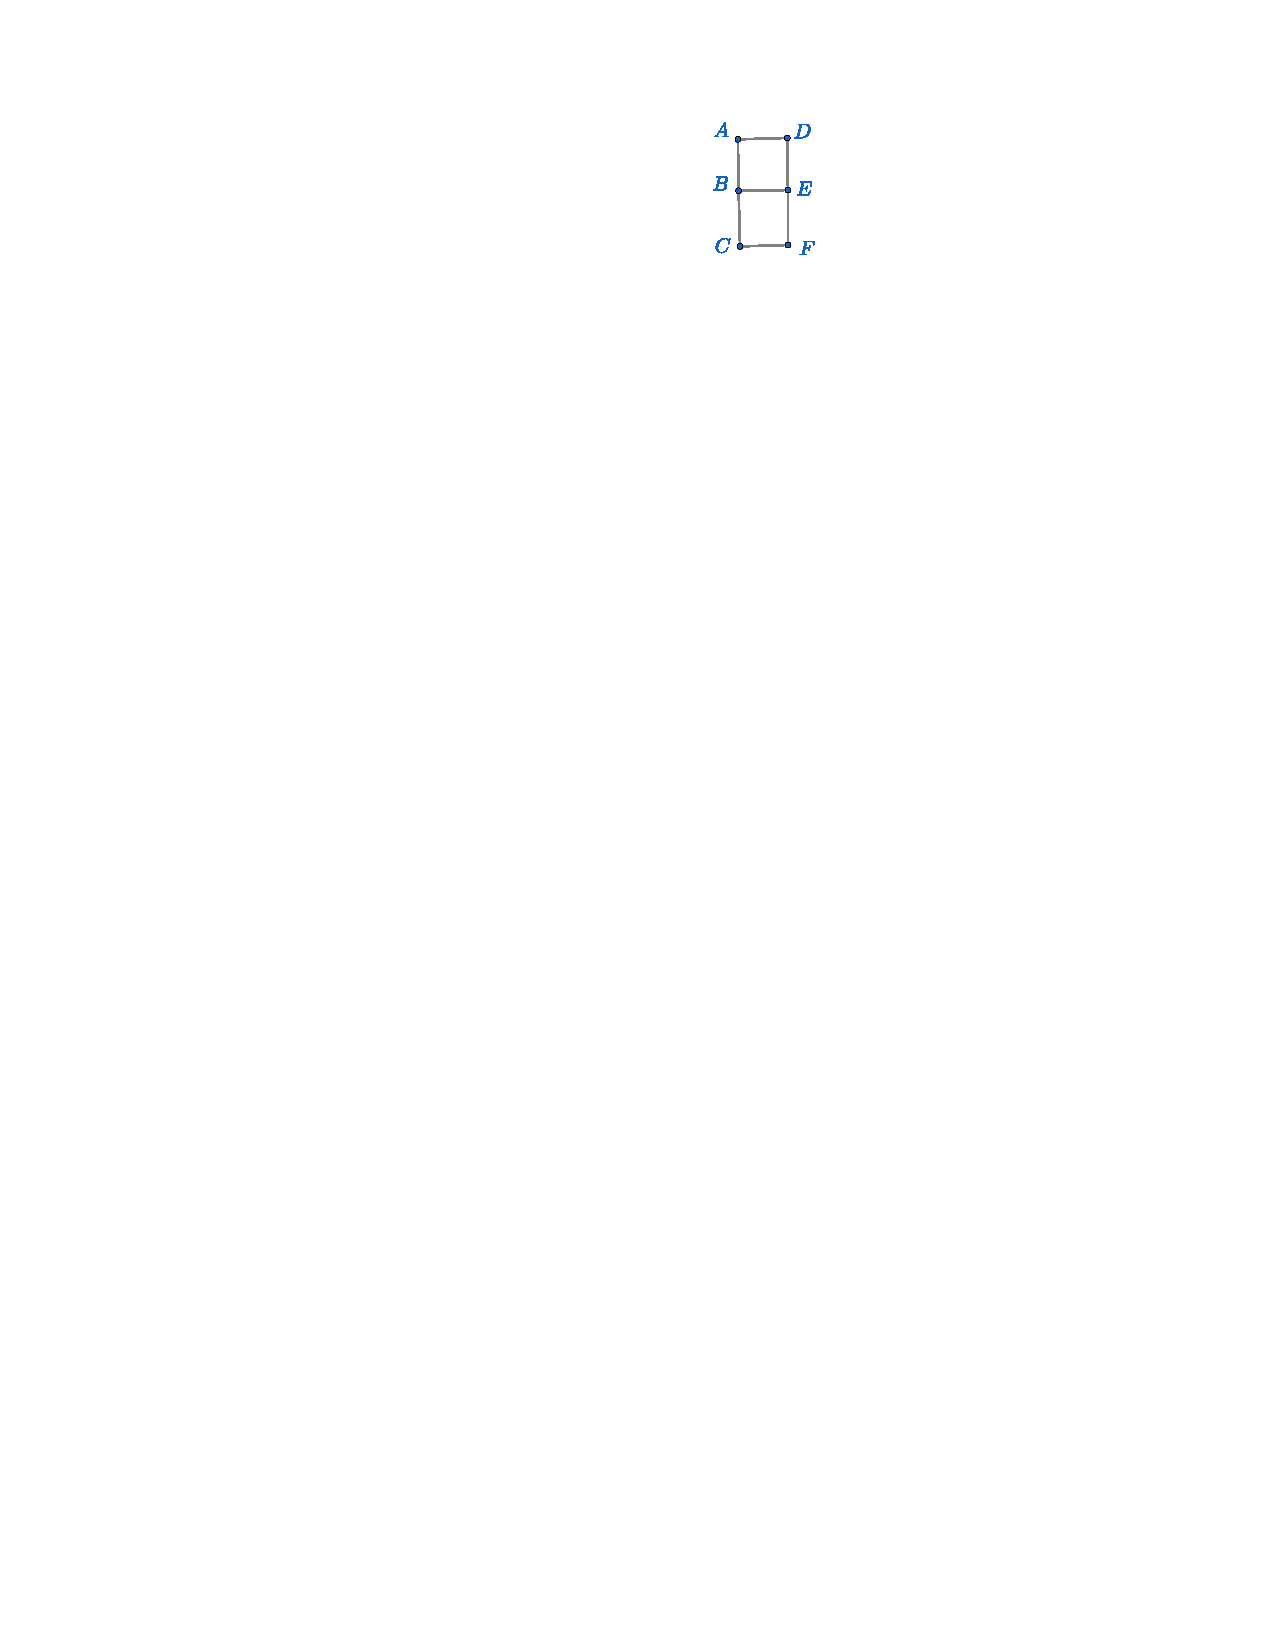
\includegraphics[width=\textwidth]{pics/sparse_relaxation/a_MD.pdf}
  \caption*{(a)}
 \end{minipage}
 \hspace{0.08\textwidth}
 \begin{minipage}[t]{0.15\textwidth}
  \centering
  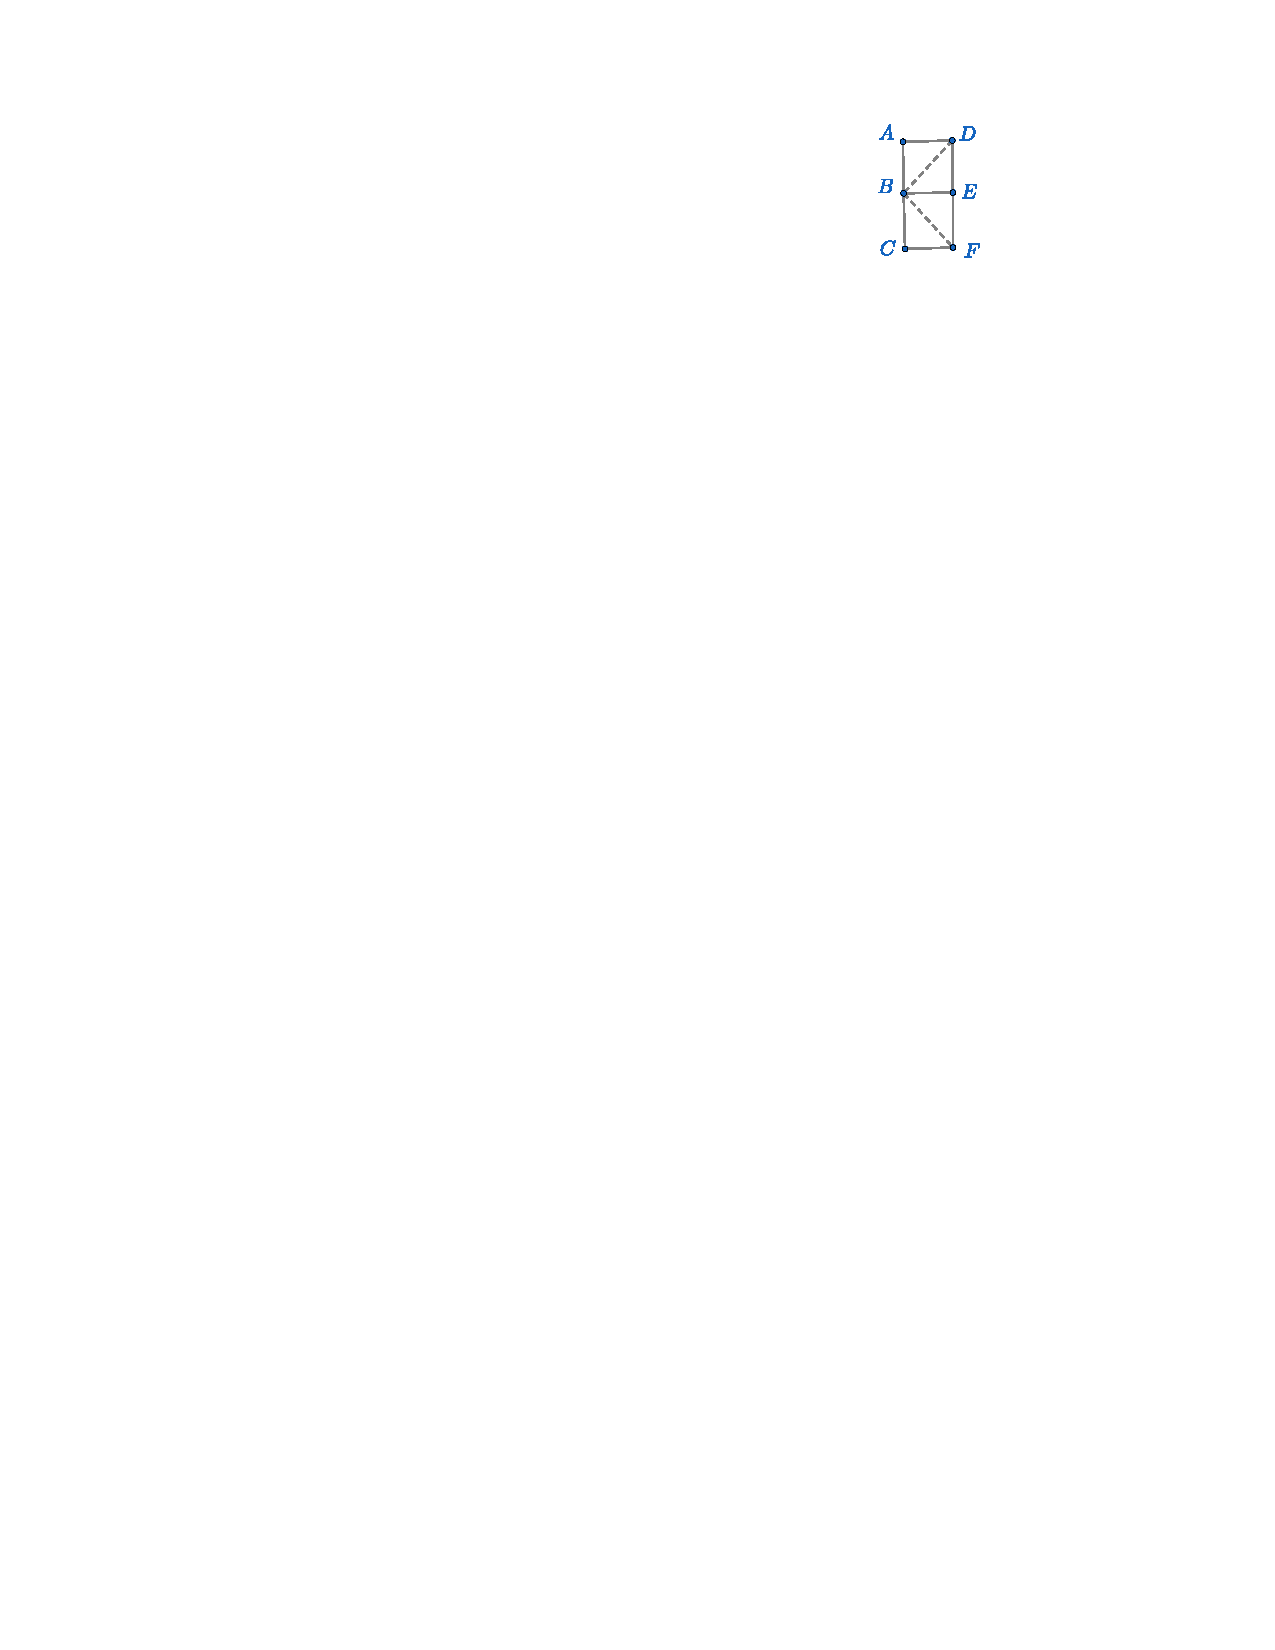
\includegraphics[width=\textwidth]{pics/sparse_relaxation/b_MD.pdf}
  \caption*{(b)}
 \end{minipage}
 \hspace{0.08\textwidth}
 \begin{minipage}[t]{0.15\textwidth}
  \centering
  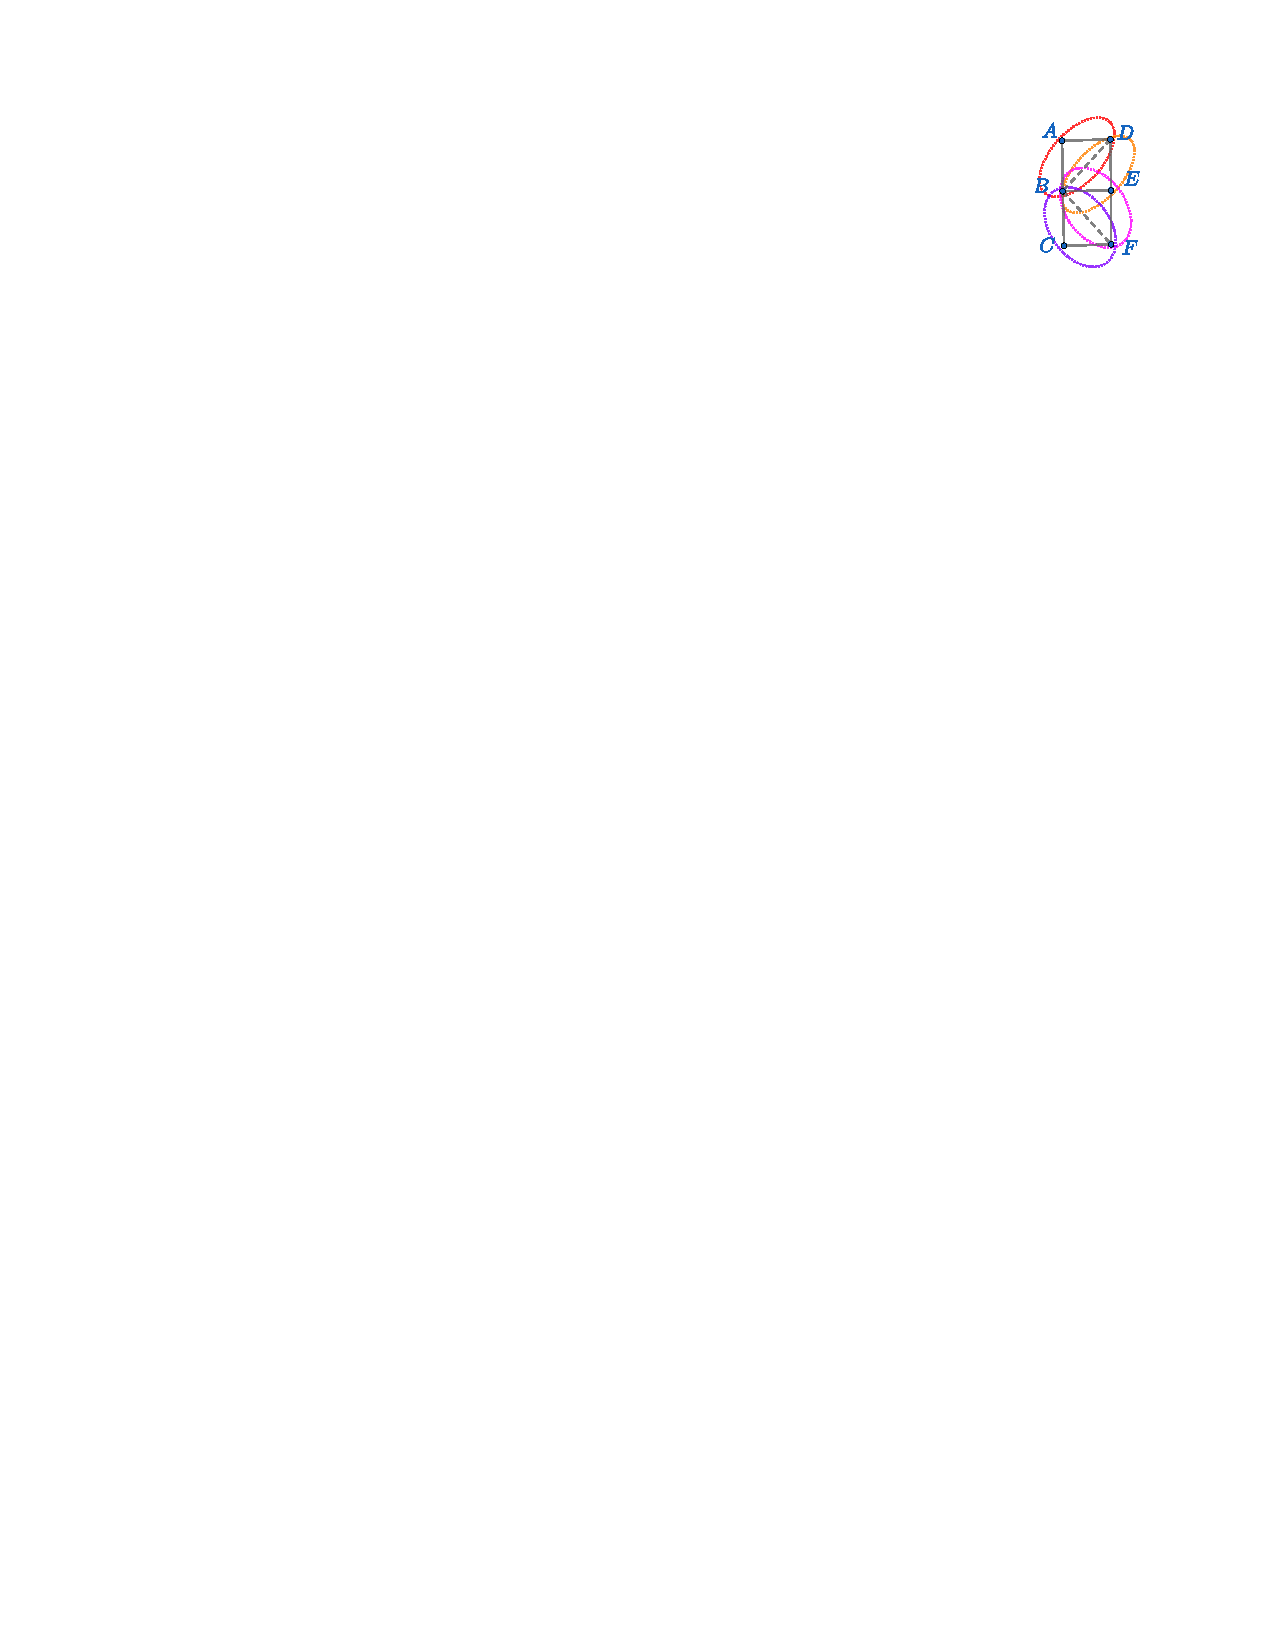
\includegraphics[width=\textwidth]{pics/sparse_relaxation/c_MD.pdf}
  \caption*{(c)}
 \end{minipage}
 \caption{An example of a chordal extension and its maximal cliques. (a) non-chordal. 
 (b) MD chordal extension. (c) maximal cliques. Adapted
 from \cite{Kang_2025Global}.}
 \label{fig:chordal_extension_cliques}
\end{figure}

\paragraph{Chain-like sparsity of trajectory optimization}
For the motion planning formulation of Section 
\ref{sec:discrete_motion_planning_of_rigid_body_systems}, the vectorized 
decision variables can be ordered as
\begin{equation}
    \bm{z}=
    \begin{bmatrix}
    \bm{Y}_0&
    \bm{U}_1&
    \bm{\lambda}_1&
    \bm{Y}_1&
    \cdots&
    \bm{U}_N&
    \bm{\lambda}_N&
    \bm{Y}_N
    \end{bmatrix}^{\top}.
 \label{eq:trajectory_decision_vector}
\end{equation}
\cite{Kang_2026Fast} defines the index set \(\mathcal I_k\), which 
selects the scalar variables of the \(k\)-th
trajectory clique,
\begin{equation}
 \bm{z}(\mathcal I_k)=
 \begin{bmatrix}
 \bm{Y}_{k-1}&\bm{U}_k&\bm{\lambda}_k&\bm{Y}_k
 \end{bmatrix}^{\top},
 \qquad k=1,\ldots,N.
 \label{eq:trajectory_clique}
\end{equation}
For multibody rigid-body systems, each link constraint 
and stage cost for transition \(k\) is contained inside \(\mathcal I_k\).
Additionally, the temporal cliques satisfy
\begin{equation}
 \bigcup_{k=1}^{N} \mathcal I_k=\{1,\ldots,n_z\},
 \qquad
 \left(\bigcup_{i=1}^{k-1}\mathcal I_i\right)\cap \mathcal I_k
 =\mathcal I_{k-1}\cap \mathcal I_k,
 \quad k=2,\ldots,N.
 \label{eq:chain_sparsity_condition}
\end{equation}
Their adjacent overlap contains the shared boundary state \(\bm{Y}_{k-1}\). Therefore,
the property \eqref{eq:chain_sparsity_condition} results from the Markov structure 
of the discretized dynamics
\cite{Sangli2025}.

Figure~\ref{fig:temporal_clique_sparsity} illustrates the chain-like sparsity
pattern for the clique \eqref{eq:trajectory_clique} and the
resulting multi-block SDP, forming a chain-like graph. Thereby,
\(\psi(\bm{Y}_{k-1},\bm{U}_k,\bm{\lambda}_k)\) denotes the stage cost,
\(\mathcal{D}(\bm{Y}_k,\bm{Y}_{k-1},\bm{U}_k,\bm{\lambda}_k)=0\) the polynomial
equality constraints, and \(H(\bm{Y}_k,\bm{U}_k,\bm{\lambda}_k)\geq0\) the polynomial inequality constraints.

\begin{figure}[!ht]
 \centering
 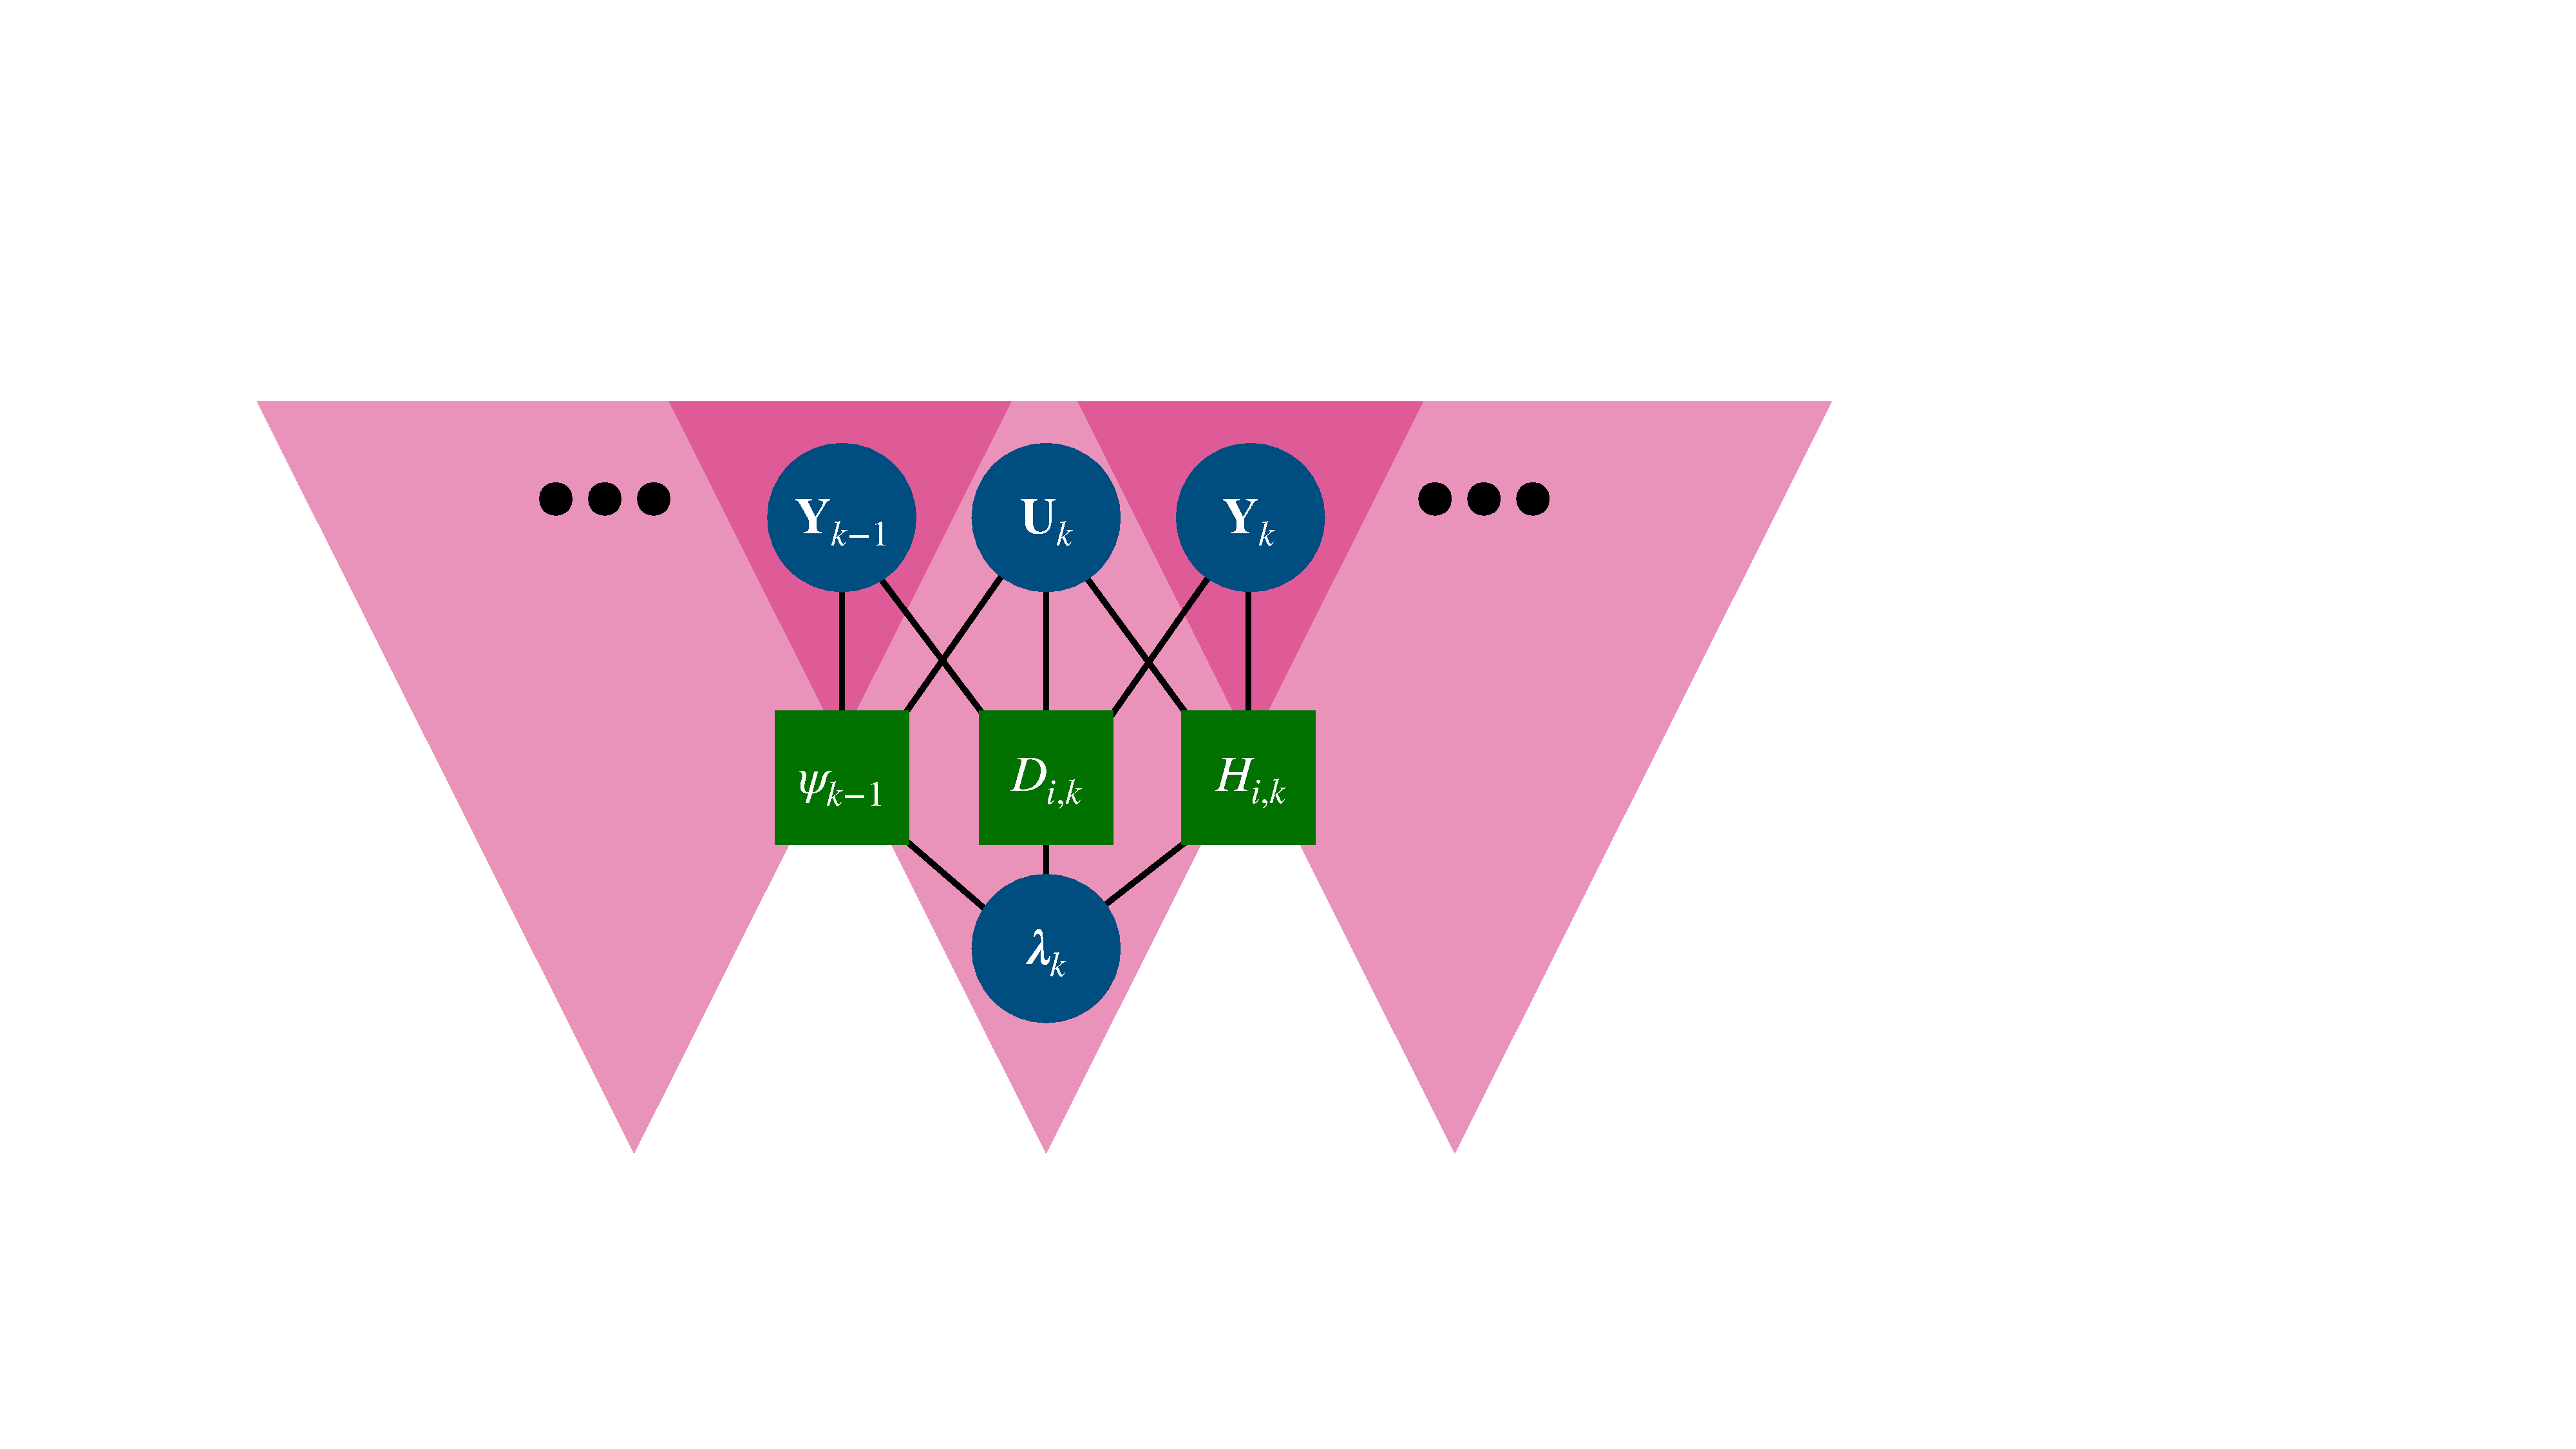
\includegraphics[width=0.6\textwidth]
 {./pics/sparse_relaxation/I_k.pdf}
 \caption{Illustration of a chain-like sparsity pattern.
 Adapted from \cite{Kang_2026Fast}.}
 \label{fig:temporal_clique_sparsity}
\end{figure}

\paragraph{Multibody rigid-body-specific sparsity}
Many robotic systems have local dependencies. 
\cite{Kang_2025Global} gives the example of a 
one-dimensional two-link chain in discrete time 
with the three states $x_{1,k}, x_{2,k}, x_{3,k}$ and the corresponding
control inputs $u_{1,k},u_{2,k},u_{3,k}$,
\begin{align}
&x_{1,k+1} = x_{1,k}+u_{1,k},\\
&x_{2,k+1} = x_{2,k}+u_{2,k},\\
&x_{3,k+1} = x_{3,k}+u_{3,k},\\
&(x_{1,k}-x_{2,k})^2 = r^2, \\
&(x_{2,k}-x_{3,k})^2 = r^2.
\end{align}
Using the chain-like sparsity condition
\eqref{eq:chain_sparsity_condition} therefore gives the nine-variable clique vector
\begin{equation}
\bm{z}(\mathcal I_k^{\mathrm{full}})
=
\begin{bmatrix}
x_{1,k}&x_{2,k}&x_{3,k}&x_{1,k+1}&x_{2,k+1}&x_{3,k+1}&u_{1,k}&u_{2,k}&u_{3,k}
\end{bmatrix}^{\top}.
\end{equation}
\cite{Kang_2025Global} elaborates that each input affects only its corresponding 
state and the geometric constraints couple only neighboring states.
Therefore, this clique vector can be decomposed further into
\begin{align}
\bm{z}(\mathcal I_{\mathrm{dyn},i,k})
&=\begin{bmatrix}x_{i,k}&x_{i,k+1}&u_{i,k}\end{bmatrix}^{\top},
&&i=1,2,3,\\
\bm{z}(\mathcal I_{\mathrm{geom},i,m})
&=\begin{bmatrix}x_{i,m}&x_{i+1,m}\end{bmatrix}^{\top},
&&i=1,2,\quad m\in\{k,k+1\}.
\end{align}
In consequence, the original clique of size nine is replaced by three 
cliques of size three and four cliques of size two.

\paragraph{Sparse Moment--SOS relaxation}
After defining the \(N_{\mathrm{cl}}\) variable cliques
\(\mathcal I_1,\ldots,\mathcal I_{N_{\mathrm{cl}}}\),
\(p(\bm{z})=\sum_{i=1}^{N_{\mathrm{cl}}}p_i(\bm{z}(\mathcal I_i))\) and every
constraint polynomial is assigned to a clique containing all of its variables,
the $\kappa$-order moment relaxation problem \eqref{eq:moment_relaxation_comparison}
can be solved. For the sparse Moment-SOS relaxation, the moment and
localizing conditions are imposed separately on the local monomial bases \cite{Kang_2025Global}.
Consequently, instead of one matrix of dimension
\(\binom{n_z+\kappa}{\kappa}\), the sparse relaxation contains blocks of
dimension \(\binom{|\mathcal I_i|+\kappa}{\kappa}\). Using the chain-like cliques
\eqref{eq:trajectory_clique}, its size remains independent of \(N\) if the
per-stage model size is fixed. Only the number of blocks grows linearly with
\(N\) \cite{Kang_2026Fast}.

Figure~\ref{fig:dense_sparse_moment_comparison} illustrates an example from
\cite{Kang_2025Global}: a reduction for
a POP with two variables \(\bm{x}=(x_1,x_2)\) and relaxation order
\(\kappa=2\). The dense moment matrix has dimension
\(\binom{2+2}{2}=6\). If the variables are separated into the cliques
\(\{x_1\}\) and \(\{x_2\}\), the sparse relaxation instead contains two moment
matrices of dimension \(\binom{1+2}{2}=3\). Consequently, one \(6\times6\)
positive-semidefinite constraint is replaced by two \(3\times3\)
positive-semidefinite constraints \cite{Kang_2025Global}.

\begin{figure}[!ht]
 \centering
 \begin{minipage}[t]{0.44\textwidth}
  \centering
  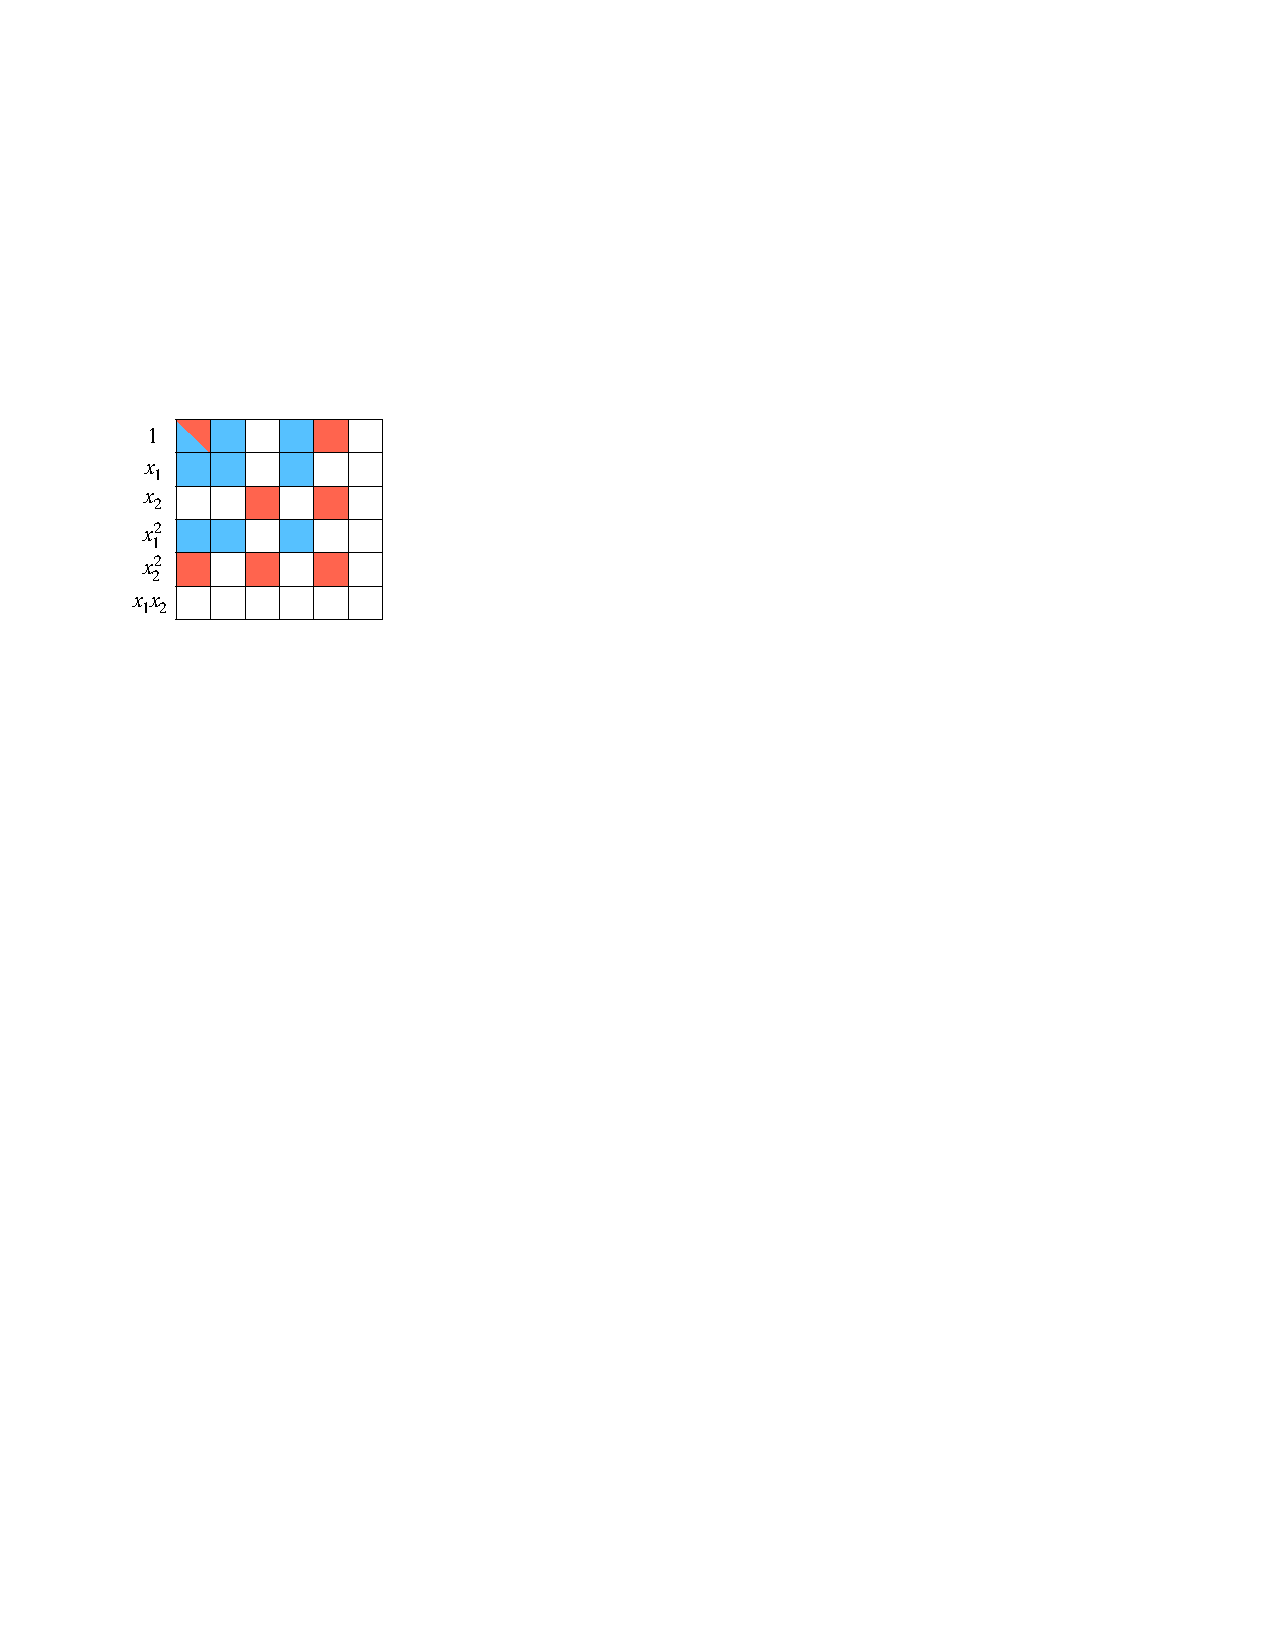
\includegraphics[width=\textwidth]{pics/sparse_relaxation/dense_moment_relaxation.pdf}
  \caption*{(a) Dense Moment Relaxation}
 \end{minipage}
 \begin{minipage}[t]{0.25\textwidth}
  \centering
  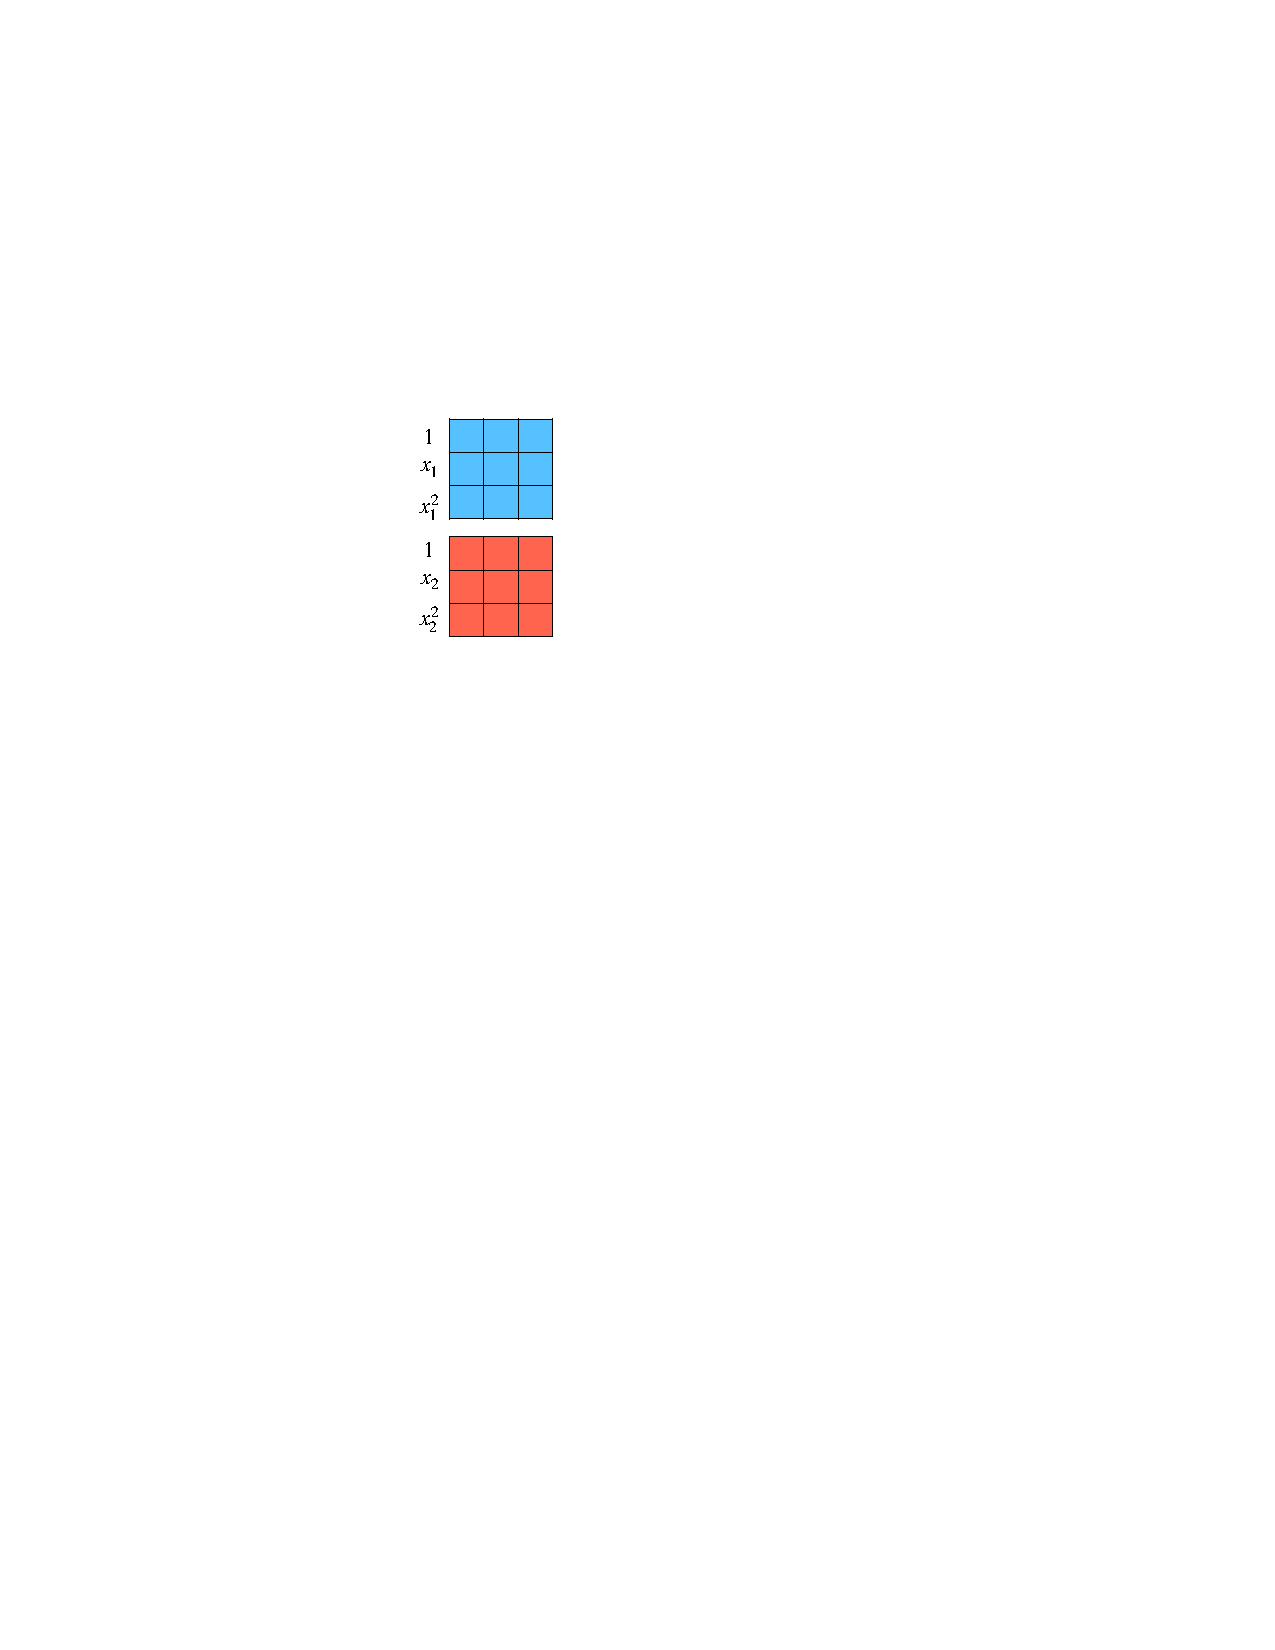
\includegraphics[width=\textwidth]{pics/sparse_relaxation/sparse_moment_relaxation.pdf}
  \caption*{(b) Sparse Moment Relaxation}
 \end{minipage}
 \caption{Comparison of dense and sparse moment matrices for a two-variable POP
 at relaxation order \(\kappa=2\). Reproduced from
 \cite{Kang_2025Global}.}
 \label{fig:dense_sparse_moment_comparison}
\end{figure}

At a fixed order $\kappa$, the sparse lower-bound may
be further away from the optimal solution $p^*$ than the dense bound. 
Still, if all optimal clique moment matrices have rank one, a globally optimal 
trajectory $\bm{z}^*$ can be extracted. However, rank one of only the first
clique does not certify the complete horizon. Following \cite{Sangli2025}, proximity to rank one is
evaluated by
\begin{equation}
 \delta_k:=\frac{\nu_{2,k}}{\nu_{1,k}},
 \qquad
 \delta_{\max}:=\max_{k=1,\ldots,N_{\mathrm{cl}}}\delta_k.
 \label{eq:numerical_rank_metric}
\end{equation}
Here, 
\(\nu_{1,k}\geq\nu_{2,k}\geq\cdots\geq0\) are the eigenvalues of
\(\bm{M}_{\kappa,k}\). \(\delta_{\max}\) close to zero indicates an approximately rank-one solution.
 Nevertheless, it remains a numerical tightness diagnostic and is not an exact certificate.

\paragraph{Sparse Polynomial Optimization Toolbox (SPOT)}
The sparse Moment--SOS relaxations in this thesis are constructed 
using the Sparse Polynomial Optimization Toolbox (SPOT) developed by 
\cite{Kang_2025Global}. Given a POP, SPOT automatically constructs its 
correlative sparsity graph, applies a chordal extension, identifies 
the maximal variable cliques, groups the polynomial constraints, and 
generates the corresponding sparse moment or SOS relaxation. For both 
CS and TS, SPOT provides maximal (MAX), minimum-degree (MD), and minimum-fill 
(MF) chordal-extension options, as well as user-defined (SELF) cliques. TS further 
decomposes the monomial bases within the variable cliques, but is not considered 
in this thesis, because of limited computational capabilities. 
In this thesis, the controlled 3D-pendulum of Section \ref{sec:discrete_3D_pendulum} uses automatic CS with the MD 
extension, whereas the Acrobot of Section \ref{subsection:discrete_Acrobot} uses problem-specific SELF cliques. 
Their exact clique constructions and relaxation orders are specified 
in the following sections.

\newpage

\section{Discrete Motion Planning for the 3D-Pendulum}
\label{sec:discrete_motion_planning_3d_pendulum}

In order to optimize the trajectory of the 3D pendulum, the discrete motion planning 
problem \eqref{eq:general_motion_optimization} has to be formulated as a 
polynomial optimization problem (POP), using the derived discrete Lie group dynamics of the
3D pendulum in Section~\ref{sec:discrete_3D_pendulum}. The optimization variables are the entries of
\(\bm{R}_0,\ldots,\bm{R}_N\), \(\bm{F}_0,\ldots,\bm{F}_{N-1}\), and the control parameters
\(\bm{u}_{p,1},\ldots,\bm{u}_{p,N-1}\), given \cite{Lee2008} definition of the control moment
\begin{equation}
    \bm{u}_k=\bm{R}_k^{\top}\bm{e}_3\times \bm{u}_{p,k}.
\end{equation}
For improved numerical conditioning, the variables have to be scaled to the range \([-1,1]\). 
Therefore, the control input is scaled by the scalar control limit as

\begin{equation}
    \bm{u}_{p,k}
    =u_{\max}\bar{\bm{u}}_{p,k},
    \qquad
    u_{\max}>0,
    \label{eq:u_scaling_3d_pendulum}
\end{equation}
so that the normalized Euclidean control bound becomes
\begin{align}\label{eq:u_bound_3d_pendulum}
    1-\bar{\bm{u}}_{p,k}^{\top}\bar{\bm{u}}_{p,k}\geq0.
\end{align}
In contrast, the entries of \(\bm{R}_k\) and \(\bm{F}_k\) are already bounded by the Lie-group constraints 
\eqref{eq:so3_polynomial_constraints}.

\cite{Kang_2026Fast} defines the cost function as a weighted sum of the terminal and stage costs 
\begin{equation}
    \begin{aligned}
    J_{\mathrm{LQR}}
    &=
    P_f
    \left(\bm{x}_N-\bm{x}_f\right)^\top
    \bm{Q}_x
    \left(\bm{x}_N-\bm{x}_f\right)
    \\
    &\quad+
    \sum_{k=0}^{N-1}
    \left\{
    \left(\bm{x}_k-\bm{x}_f\right)^\top
    \bm{Q}_x
    \left(\bm{x}_k-\bm{x}_f\right)
    +
    \bm{u}_k^\top \bm{Q}_u \bm{u}_k
    \right\},
    \end{aligned}
    \label{eq:lqr_style_loss}
\end{equation}
where $\bm{Q}_x$ and $\bm{Q}_u$ are the identity matrices after rescaling of the variables. 
In addition to \eqref{eq:lqr_style_loss}, this thesis uses individual weights $w_R$, $w_F$ for
the terminal costs and $\alpha_R$, $\alpha_F$, $w_u$ for
the stage costs.  

In the next step, the constraints given by \eqref{eq:general_motion_optimization} have to be 
identified for the 3D-pendulum. The equality constraints $\mathcal{D}$ are given by the discrete 
forced dynamics \eqref{eq:forced_3D_pendulum_EL_dynamics} and the 
kinematics update \eqref{eq:forced_3D_pendulum_EL_kinematics}. Moreover, the
Lie-group constraints $\mathcal{Y}$ defined in Section~\ref{sec:discrete_motion_planning_of_rigid_body_systems}
by \eqref{eq:so3_polynomial_constraints} have to be included for $\bm{R}_k$ and $\bm{F}_k$.
Finally, by using the inequality relation $\mathcal{H}$ given in \cite{GallierQuaintance2020LinearAlgebra}, 
\begin{align}
    \operatorname{tr}(\bm{F}_k)=1+2\cos(\Delta\theta_k)
\end{align}
the relative rotation during one step $\bm{F}_k$ is bounded by the angle $0 \leq \Delta\theta_{\max} \leq \pi$, and
the control input by \eqref{eq:u_bound_3d_pendulum}. In summary, the full controlled 
3D-pendulum POP is defined as
\begingroup
\footnotesize
\begin{subequations}
\label{eq:controlled_3d_pendulum_pop}
\begin{align}
p_{\mathrm{P}}^{\star}
=
\min_{\substack{
\{\bm{R}_k\}_{k=0}^{N},\,\{\bm{F}_k\}_{k=0}^{N-1}\\[-0.2em]
\{\bar{\bm{u}}_{p,k}\}_{k=1}^{N-1}}}
\quad
&w_R\left\|\bm{R}_N-\bm{R}_N^{\mathrm{des}}\right\|_F^2
+w_F\left\|\bm{F}_{N-1}-\bm{F}^{\mathrm{des}}\right\|_F^2
\notag\\[-0.9em]
&+\alpha_R \sum_{k=0}^{N-1}
\left\|\bm{R}_k-\bm{R}_N^{\mathrm{des}}\right\|_F^2
+\alpha_F \sum_{k=0}^{N-2}
\left\|\bm{F}_k-\bm{F}^{\mathrm{des}}\right\|_F^2
\notag\\[0.4em]
&+\frac{1}{w_u} \sum_{k=1}^{N-1}\left\|\bar{\bm{u}}_{p,k}\right\|_2^2
\label{eq:controlled_3d_pendulum_pop_objective}
\\[0.2em]
\hspace{-0.9em}\text{s.t.}\quad
&\hspace{-0.9em}\begin{aligned}
\frac{1}{h}\left(
\bm{F}_{k+1}\bm{J}_d-\bm{J}_d\bm{F}_{k+1}^{\top}-\bm{J}_d\bm{F}_k+\bm{F}_k^{\top}\bm{J}_d
\right)
&=h\left(\bm{\tau}_{g,k+1}+\bm{u}_{k+1}\right)^{\wedge}
\end{aligned},
\label{eq:controlled_3d_pendulum_pop_dynamics}
\\[0.8em]
&\hspace{-0.9em}\begin{aligned}
\bm{R}_{k+1}&=\bm{R}_k\bm{F}_k
\end{aligned},
\label{eq:controlled_3d_pendulum_pop_kinematics}
\\[0.8em]
&\hspace{-0.9em}\begin{aligned}
&\|\bm{r}_{1,k}\|_2^2-1=\|\bm{r}_{2,k}\|_2^2-1=\|\bm{r}_{3,k}\|_2^2-1=0,\\[-0.2em]
&\bm{r}_{1,k}^{\top}\bm{r}_{2,k}=\bm{r}_{2,k}^{\top}\bm{r}_{3,k}
=\bm{r}_{1,k}^{\top}\bm{r}_{3,k}=0,\\[-0.2em]
&\bm{r}_{1,k}\!\times \bm{r}_{2,k}-\bm{r}_{3,k}
=\bm{r}_{2,k}\!\times \bm{r}_{3,k}-\bm{r}_{1,k}
=\bm{r}_{3,k}\!\times \bm{r}_{1,k}-\bm{r}_{2,k}=\bm{0}_{3\times1},
\end{aligned}
\label{eq:controlled_3d_pendulum_pop_so3_R}
\\[0.8em]
&\hspace{-0.9em}\begin{aligned}
&\|\bm{f}_{1,k}\|_2^2-1=\|\bm{f}_{2,k}\|_2^2-1=\|\bm{f}_{3,k}\|_2^2-1=0,\\[-0.2em]
&\bm{f}_{1,k}^{\top}\bm{f}_{2,k}=\bm{f}_{2,k}^{\top}\bm{f}_{3,k}
=\bm{f}_{1,k}^{\top}\bm{f}_{3,k}=0,\\[-0.2em]
&\bm{f}_{1,k}\!\times \bm{f}_{2,k}-\bm{f}_{3,k}
=\bm{f}_{2,k}\!\times \bm{f}_{3,k}-\bm{f}_{1,k}
=\bm{f}_{3,k}\!\times \bm{f}_{1,k}-\bm{f}_{2,k}=\bm{0}_{3\times1},
\end{aligned}
\label{eq:controlled_3d_pendulum_pop_so3_F}
\\[0.8em]
&\hspace{-0.9em}\begin{aligned}
\frac{\operatorname{tr}(\bm{F}_k)-1}{2}
&\geq \cos(\Delta\theta_{\max})
\end{aligned},
\label{eq:controlled_3d_pendulum_pop_step_bound}
\\[0.8em]
&\hspace{-0.9em}\begin{aligned}
1-\bar{\bm{u}}_{p,k}^{\top}\bar{\bm{u}}_{p,k}&\geq0
\end{aligned},
\label{eq:controlled_3d_pendulum_pop_control_bound}
\\[0.8em]
&\hspace{-0.9em}\begin{aligned}
\bm{R}_0&=\bm{R}^{\mathrm{init}},
\qquad \bm{F}_0=\bm{F}^{\mathrm{init}}
\end{aligned}.
\label{eq:controlled_3d_pendulum_pop_initial}
\end{align}
\end{subequations}
\endgroup
with the initial conditions \(\bm{R}^{\mathrm{init}}\) and \(\bm{F}^{\mathrm{init}}\).
Here, \eqref{eq:controlled_3d_pendulum_pop_dynamics} holds for
\(k=0,\ldots,N-2\), \eqref{eq:controlled_3d_pendulum_pop_kinematics}
and \eqref{eq:controlled_3d_pendulum_pop_step_bound} hold for
\(k=0,\ldots,N-1\), \eqref{eq:controlled_3d_pendulum_pop_so3_R}
holds for \(k=0,\ldots,N\), \eqref{eq:controlled_3d_pendulum_pop_so3_F}
holds for \(k=0,\ldots,N-1\), and
\eqref{eq:controlled_3d_pendulum_pop_control_bound} holds for
\(k=1,\ldots,N-1\).
Moreover, \(h\) is the time step, \(\bm{J}_d\) is the nonstandard inertia matrix \eqref{eq:non-standard_inertia},
and $\bm{\tau}_{g,k}$ denotes the gravity moment in the body-fixed frame \eqref{eq:3d_pendulum_gravity_moment}.
The definition of \(\bm{r}_{i,k}\) and \(\bm{f}_{i,k}\) is given in \eqref{eq:so3_polynomial_constraints}.
Finally, \eqref{eq:controlled_3d_pendulum_pop} gives the full POP of the 3d-pendulum with 
polynomials until degree 2.

In order to construct the sparse moment relaxation, the chain-like sparsity 
structure of the 3D-pendulum POP has to be identified. The local decision vector
associated with the pendulum clique index set \(\mathcal I_k^{\mathrm{P}}\) is ordered as
\begin{align}\label{eq:3d_pendulum_sparse_clique}
    \bm{z}_{\mathrm{P}}(\mathcal I_k^{\mathrm{P}})
    =
    [\bm{R}_{k+1} \quad \bm{F}_{k+1} \quad \bm{R}_{k} \quad \bm{F}_{k} \quad \bar{\bm{u}}_{p,k+1} ]^{\top},
    \qquad k=0,\ldots,N-2,
\end{align}
which is consistent with the chain-like sparsity condition \eqref{eq:chain_sparsity_condition}.
Thereby, the dynamics and kinematics only couple neighboring time steps. 
Therefore, the clique vector \(\bm{z}_{\mathrm{P}}(\mathcal I_k^{\mathrm{P}})\)
contains \(n_{\mathrm{cl}}=39\) scalar variables.
\cite{Sangli2025} identifies for a clique size of \(n_{\mathrm{cl}}\), the order-\(\kappa\) moment matrix
dimension as
\begin{equation}
s(n_{\mathrm{cl}},\kappa)
=\binom{n_{\mathrm{cl}}+\kappa}{\kappa}.
\label{eq:moment_size}
\end{equation}
Consequently, at $\kappa=2$, a 39-variable interior clique
\(\bm{z}_{\mathrm{P}}(\mathcal I_k^{\mathrm{P}})\) yields $s(39,2)=820$.
The corresponding moment matrix therefore has size $820\times820$. In
contrast, the full decision vector contains
\[
 n_{z,\mathrm{P}}=9(N+1)+9N+3(N-1)=21N+6
\]
variables. A dense second-order relaxation would consequently require a moment
matrix of size
\[
s(n_{z,\mathrm{P}},2)=\binom{21N+8}{2}.
\]
For the implemented horizon $N=20$, this corresponds to a
$91\,378\times91\,378$ moment matrix, which is computationally not feasible. 
Nevertheless, the spare relaxation \eqref{eq:3d_pendulum_sparse_clique} 
consists of bigger miment matrices, compared to the moment matrices constructed using 
MD, which will be used for the Evaluation.
In the following Section \ref{sec:3d_pendulum_optimization_results},
SPOT is used to construct the second-order sparse moment relaxation from the 3D-pendulum's POP 
\eqref{eq:controlled_3d_pendulum_pop} \cite{Kang_2025Global}. The resulting SDP is solved with the interior-point solver
MOSEK \cite{MOSEK}. The scalar equations used in the implementation are listed in
Appendix~\ref{app:controlled_3d_pendulum_scalar_pop}. Finally, the implementation is documented 
in the GitHub repository \cite{Elshani2026CTO_GitHub}.

\section{Discrete Motion Planning for an Acrobot}
\label{sec:discrete_motion_planning_acrobot}

The following section applies the discrete motion planning formulation of
Section \ref{sec:discrete_motion_planning_of_rigid_body_systems} 
to the controlled Acrobot derived in Section \ref{subsection:discrete_Acrobot}. 
First, the trajectory optimization problem is solved in Section 
\ref{sec:trajectory_optimization_via_sdp_relaxation} 
using a sparse semidefinite relaxation. Subsequently, the same relaxation is 
embedded into a model predictive control framework to obtain a 
closed-loop controller in Section \ref{sec:acrobot_trajectory_optimization_SDP_MPC}.

\subsection{Trajectory Optimization via SDP Relaxation}
\label{sec:trajectory_optimization_via_sdp_relaxation}
To optimize the Acrobot trajectory, the discrete motion planning
problem \eqref{eq:general_motion_optimization} has to be formulated as a POP using
the controlled discrete Euler-Lagrange equations of Section \ref{subsection:discrete_Acrobot}. 
For the two links $i=1,2$, the planar rotations are represented around the z-axis by 
\eqref{eq:so2_polynomial_constraints}.
The Acrobot model in maximal coordinates contains additional 
velocity variables $\bm{v}_{i,k}\in\mathbb R^2$, which results in a higher number of optimization variables.
Instead, the maximal coordinate model can be reduced by eliminating the
translational positions and velocities while the constraints still remain
polynomial. Therefore, the 
holonomic constraints \eqref{eq:acrobot_base_constraint} and 
\eqref{eq:acrobot_elbow_constraint} eliminate the center-of-mass
positions exactly according to
\begin{equation}
\bm{x}_{1,k}=\bm{p}_0-\bm{R}_{1,k}\bm{\rho}_{1,0},
\qquad
\bm{x}_{2,k}=\bm{p}_0+\bm{R}_{1,k}(\bm{\rho}_{1,12}-\bm{\rho}_{1,0})
               -\bm{R}_{2,k}\bm{\rho}_{2,12}.
\label{eq:acrobot_eliminated_positions}
\end{equation}
Therefore, the velocity $\bm{v}_{i,k}$ can be approximated from the rotations by  
\begin{subequations}\label{eq:velocity_approximation_rotations}
\begin{align}
    \bm{v}_{1,k}
    &\approx
    \frac{(\bm{R}_{1,k}-\bm{R}_{1,k+1})\bm{\rho}_{1,0}}{h},
    \label{eq:velocity_approximation_link1}\\
    \bm{v}_{2,k}
    &\approx
    \frac{
        (\bm{R}_{1,k+1}-\bm{R}_{1,k})
        (\bm{\rho}_{1,12}-\bm{\rho}_{1,0})
        -(\bm{R}_{2,k+1}-\bm{R}_{2,k})\bm{\rho}_{2,12}
    }{h}.
    \label{eq:velocity_approximation_link2}
\end{align}
\end{subequations}
substituting \eqref{eq:acrobot_eliminated_positions} into \eqref{eq:acrobot_discrete_translational_velocity}.
In addition, the kinematic update \eqref{eq:acrobot_full_del_shifted_kinematics_1}-\eqref{eq:acrobot_full_del_shifted_kinematics_2} can be rewritten as
\begin{equation}
\bm{R}_{i,k-1}=\bm{R}_{i,k}\bm{F}_{i,k-1}^{\top}.
\label{eq:acrobot_kinematic_substitution}
\end{equation}
Consequently, using \eqref{eq:acrobot_full_del_shifted_kinematics_1}-\eqref{eq:acrobot_full_del_shifted_kinematics_2},
\eqref{eq:acrobot_kinematic_substitution} and \eqref{eq:velocity_approximation_rotations},
the translational dynamics 
\eqref{eq:acrobot_full_del_shifted_translation_1}-\eqref{eq:acrobot_full_del_shifted_translation_2} are reduced to a polynomial form 
\begin{subequations}
\begingroup
\setlength{\jot}{0.35em}
\vspace{-0.3cm}
\begin{align}
    \intertext{\textit{Translation:}}
    \vspace{-0.1cm}
    -\bm{M}_1 \bm{R}_{1,k}
    \bm{A}_{1,k}\bm{\rho}_{1,0}
    -h^2g\bm{M}_1\bm{e}_2
    -h^2\left(\bm{\lambda}_{0,k}+\bm{\lambda}_{12,k}\right)
    &=
    \bm{0},
    \label{eq:acrobot_full_del_shifted_translation_1_reduced}
    \\
\hspace{-2em}
    \bm{M}_2\Bigl[
    \bm{R}_{1,k}
    \bm{A}_{1,k}
    \left(\bm{\rho}_{1,12}-\bm{\rho}_{1,0}\right)
    -\bm{R}_{2,k}
    \bm{A}_{2,k}\bm{\rho}_{2,12}
    \Bigr]
    -h^2g\bm{M}_2\bm{e}_2
    +h^2\bm{\lambda}_{12,k}
    &=
    \bm{0},
    \label{eq:acrobot_full_del_shifted_translation_2_reduced}
\end{align}
\endgroup
\end{subequations}
with $\bm{A}_{i,k}=\bm{F}_{i,k}-2\bm{I}_2+\bm{F}_{i,k-1}^{\top}$.
Therefore, the reduced translational dynamics only depend on the relative rotations
$\bm{F}_{i,k}$ and $\bm{F}_{i,k-1}$, and the attitude $\bm{R}_{i,k}$.
The physical properties of the reduced model are validated and compared to the full model in the 
Appendix \ref{appendix:experimental_details}.

Similar to the 3D pendulum in Section \ref{sec:discrete_motion_planning_3d_pendulum}, 
for numerical conditioning, the control and constraint multipliers are scaled
to the interval $[-1,1]$ componentwise,
\begin{equation}
u_k^{\mathrm{phys}}=u_{\max}\bar u_k,
\qquad
\bm{\lambda}_{0,k}=\lambda_{\max}\bar{\bm{\lambda}}_{0,k},
\qquad
\bm{\lambda}_{12,k}=\lambda_{\max}\bar{\bm{\lambda}}_{12,k}.
\label{eq:acrobot_variable_scaling}
\end{equation}
The normalized control and componentwise multiplier bounds are
\begin{equation}
1-\bar u_k^2\geq0,
\qquad
1-\bigl(\bar{\lambda}_{0,k}^{(j)}\bigr)^2\geq0,
\qquad
1-\bigl(\bar{\lambda}_{12,k}^{(j)}\bigr)^2\geq0,
\quad j=1,2.
\label{eq:acrobot_normalized_bounds}
\end{equation}
Moreover, since
$\tfrac12\operatorname{tr}(\bm{F}_{i,k})=a_{i,k}=\cos(\Delta\theta_{i,k})$,
the relative-rotation bound is
\begin{align}\label{eq:acrobot_normalized_f_bound}
a_{i,k}\geq\cos(\Delta\theta_{i,\max}).
\end{align} 
The entries of $\bm{R}_{i,k}$ and
$\bm{F}_{i,k}$ are already bounded by the $SO(2)$ constraints.

The optimization variables are the entries of
$\bm{R}_{i,0},\ldots,\bm{R}_{i,N}$, $\bm{F}_{i,0},\ldots,\bm{F}_{i,N-1}$, and the normalized
variables $\bar{\bm{\lambda}}_{0,k},\bar{\bm{\lambda}}_{12,k}\in\mathbb R^2$ and
$\bar u_k\in\mathbb R$, $k=1,\ldots,N-1$.
Therefore, the reduced full-horizon decision vector contains $n_{z,\mathrm{A}}^{reduced}=13N-1$
scalar variables, compared to the original $n_{z,\mathrm{A}}^{full}=17N+3$ variables of the full model using position variables $\bm{x_{i,k}}$.


Similar to the 3D-pendulum objective introduced in \eqref{eq:lqr_style_loss}
(see Section \ref{sec:discrete_motion_planning_3d_pendulum}), the Acrobot
objective uses individual terminal weights $w_R,w_F,$ and stage weights 
$\alpha_R,\alpha_F$, and \(w_u\). The multipliers $\bar{\bm{\lambda}}_{0,k}$ and $\bar{\bm{\lambda}}_{12,k}$ 
are not penalized. In the notation of the general problem~\eqref{eq:general_motion_optimization}, 
the equality constraints $\mathcal{D}_i$ consist of the reduced translational 
\eqref{eq:acrobot_full_del_shifted_translation_1_reduced}-\eqref{eq:acrobot_full_del_shifted_translation_2_reduced} 
and rotational dynamics \eqref{eq:forced_acrobot_rotation_link1}-\eqref{eq:forced_acrobot_rotation_link2},
together with the kinematic update 
\eqref{eq:acrobot_full_del_shifted_kinematics_1}-\eqref{eq:acrobot_full_del_shifted_kinematics_2}. 
The SO(2) Lie-group constraints \eqref{eq:so2_polynomial_constraints}
form $\mathcal{Y}_i$, whereas $\mathcal{H}$ contains the increment \eqref{eq:acrobot_normalized_f_bound},
control, and multiplier bounds \eqref{eq:acrobot_normalized_bounds}.
In summary, the
full controlled Acrobot POP is defined as
\begingroup
\footnotesize
\allowdisplaybreaks
\begin{subequations}
\label{eq:controlled_acrobot_pop}
\begin{align}
p_{\mathrm A}^{\star}
=
\min_{\bm{z}_{\mathrm{A}}}
\quad
&w_R\sum_{i=1}^{2}\|\bm{R}_{i,N}-\bm{R}_i^{\mathrm{des}}\|_F^2
+w_F\sum_{i=1}^{2}\|\bm{F}_{i,N-1}-\bm{F}_i^{\mathrm{des}}\|_F^2
\notag\\[-0.1em]
&+\alpha_R\sum_{k=0}^{N-1}\sum_{i=1}^{2}
  \|\bm{R}_{i,k}-\bm{R}_i^{\mathrm{des}}\|_F^2
+\alpha_F\sum_{k=0}^{N-2}\sum_{i=1}^{2}
  \|\bm{F}_{i,k}-\bm{F}_i^{\mathrm{des}}\|_F^2
\notag\\[-0.1em]
&+\frac{1}{w_u}\sum_{k=1}^{N-1}\bar u_k^2
\label{eq:controlled_acrobot_pop_objective}
\\[0.2em]
\hspace{-0.9em}\text{s.t.}\quad
&\hspace{-0.9em}\begin{aligned}
-\bm{M}_1 \bm{R}_{1,k}
\bm{A}_{1,k}\bm{\rho}_{1,0}
-h^2g\bm{M}_1\bm{e}_2
-h^2\left(\bar{\bm{\lambda}}_{0,k}+\bar{\bm{\lambda}}_{12,k}\right)
&=\bm{0}_2
\end{aligned}
\label{eq:controlled_acrobot_pop_translation_1}\\
&\hspace{-0.9em}\begin{aligned}
\bm{M}_2\Bigl[
\bm{R}_{1,k}
\bm{A}_{1,k}
\left(\bm{\rho}_{1,12}-\bm{\rho}_{1,0}\right)
-\bm{R}_{2,k}
\bm{A}_{2,k}\bm{\rho}_{2,12}
\Bigr]
-h^2g\bm{M}_2\bm{e}_2
+h^2\bar{\bm{\lambda}}_{12,k}
&=\bm{0}_2
\end{aligned}
\label{eq:controlled_acrobot_pop_translation_2}\\[0.8em]
&\hspace{-0.9em}\begin{aligned}
&
\hat{\bm{\Pi}}_{1,k}
-\hat{\bm{\Pi}}_{1,k+1}
\\
&\quad
+h
\left[
\left(
\bm{\rho}_{1,0}
\times
\bm{R}_{1,k+1}^{\top}\bar{\bm{\lambda}}_{0,k+1}
\right)
+
\left(
\bm{\rho}_{1,12}
\times
\bm{R}_{1,k+1}^{\top}\bar{\bm{\lambda}}_{12,k+1}
\right)
-u_{\max}\bar u_{k+1}
\right]^{\wedge}
&=\bm{0}
\end{aligned}
\label{eq:controlled_acrobot_pop_rotation_1}
\\
&\hspace{-0.9em}\begin{aligned}
\hat{\bm{\Pi}}_{2,k}
-\hat{\bm{\Pi}}_{2,k+1}
+h
\left[
u_{\max}\bar u_{k+1}
-
\left(
\bm{\rho}_{2,12}
\times
\bm{R}_{2,k+1}^{\top}\bar{\bm{\lambda}}_{12,k+1}
\right)
\right]^{\wedge}
&=\bm{0}
\end{aligned}
\label{eq:controlled_acrobot_pop_rotation_2}\\[0.8em]
&\hspace{-0.9em}\bm{R}_{i,k+1}=\bm{R}_{i,k}\bm{F}_{i,k},
\label{eq:controlled_acrobot_pop_kinematics}\\[0.8em]
&\hspace{-0.9em}c_{i,k}^2+s_{i,k}^2-1=0,
\label{eq:controlled_acrobot_pop_so2_R}\\
&\hspace{-0.9em}a_{i,k}^2+b_{i,k}^2-1=0,
\label{eq:controlled_acrobot_pop_so2_F}\\[0.8em]
&\hspace{-0.9em}a_{i,k}-\cos(\Delta\theta_{i,\max})\geq0,
\label{eq:controlled_acrobot_pop_step_bound}\\
&\hspace{-0.9em}1-\bar u_k^2\geq0,
\label{eq:controlled_acrobot_pop_control_bound}\\
&\hspace{-0.9em}1-\bigl(\bar{\lambda}_{0,k}^{(j)}\bigr)^2\geq0,
\quad
1-\bigl(\bar{\lambda}_{12,k}^{(j)}\bigr)^2\geq0,
\label{eq:controlled_acrobot_pop_multiplier_bound}\\[0.8em]
&\hspace{-0.9em}\begin{gathered}
\bm{F}_{i,0}=\bm{F}_i^{\mathrm{init}},\qquad
\bm{R}_{i,1}=\bm{R}_i^{\mathrm{init}}.
\end{gathered}
\label{eq:controlled_acrobot_pop_initial}
\end{align}
\end{subequations}
\endgroup

\begin{table}[htbp]
\centering
\small
\caption{Index ranges for the constraints in the controlled Acrobot POP.}
\label{tab:controlled_acrobot_pop_indexing}
\begin{tabular}{@{}lll@{}}
\toprule
Constraint & Equation(s) & Indexing \\
\midrule
Translation
& \eqref{eq:controlled_acrobot_pop_translation_1},
  \eqref{eq:controlled_acrobot_pop_translation_2}
& \(k=1,\ldots,N-1\) \\
Rotation
& \eqref{eq:controlled_acrobot_pop_rotation_1},
  \eqref{eq:controlled_acrobot_pop_rotation_2}
& \(k=0,\ldots,N-2\) \\
Kinematics
& \eqref{eq:controlled_acrobot_pop_kinematics}
& \(i=1,2,\; k=0,\ldots,N-1\) \\
\(SO(2)\) for \(\bm{R}\)
& \eqref{eq:controlled_acrobot_pop_so2_R}
& \(i=1,2,\; k=0,\ldots,N\) \\
\(SO(2)\) for \(\bm{F}\)
& \eqref{eq:controlled_acrobot_pop_so2_F}
& \(i=1,2,\; k=0,\ldots,N-1\) \\
Step bound
& \eqref{eq:controlled_acrobot_pop_step_bound}
& \(i=1,2,\; k=1,\ldots,N-1\) \\
Control bound
& \eqref{eq:controlled_acrobot_pop_control_bound}
& \(k=1,\ldots,N-1\) \\
Multiplier bound
& \eqref{eq:controlled_acrobot_pop_multiplier_bound}
& \(j=1,2,\; k=1,\ldots,N-1\) \\
Initial conditions
& \eqref{eq:controlled_acrobot_pop_initial}
& \(i=1,2\) \\
\bottomrule
\end{tabular}
\end{table}
Table \ref{tab:controlled_acrobot_pop_indexing} describes the index ranges for the constraints in the controlled Acrobot POP.
Since the center-of-mass positions are reconstructed from the rotations \eqref{eq:acrobot_eliminated_positions},
the holonomic constraints \eqref{eq:acrobot_full_del_shifted_base_constraint}-\eqref{eq:acrobot_full_del_shifted_elbow_constraint}
are satisfied identically and therefore do not appear in the reduced POP.
Moreover, $\bm{F}_{i,0}=\bm{F}_i^{\mathrm{init}}$ and
$\bm{R}_{i,1}=\bm{R}_i^{\mathrm{init}}$ specify the initial rotation increment and attitude of each link, respectively.
Instead of using fixed boundary conditions, the desired terminal values are penalized. 
Finally, the full POP of the Acrobot on $SO(2)$ in~\eqref{eq:controlled_acrobot_pop} 
is a polynomial of degree less than or equal to two.

\paragraph{Chain-like sparsity}
The reduced dynamics and kinematics couple neighboring time steps.
Following the chain-like sparsity pattern introduced in Section 
\ref{sec:semidefinite_optimization_relaxation}, the first
complete stage clique is
\begin{equation}
\hspace{-1.3em}
\begin{aligned}
\bm{z}_{\mathrm{A}}(\mathcal I_1^{\mathrm{A}})
=
\left[
\bm{R}_{1,0},\bm{R}_{2,0},
\bm{R}_{1,1},\bm{R}_{2,1},
\bm{R}_{1,2},\bm{R}_{2,2},
\bm{F}_{1,0},\bm{F}_{2,0},
\bm{F}_{1,1},\bm{F}_{2,1},
\bar{\bm{\lambda}}_{0,1},
\bar{\bm{\lambda}}_{12,1},
\bar u_1
\right]^{\top},
\end{aligned}
\label{eq:acrobot_full_self_initial_clique}
\end{equation}
whereas the remaining complete stage cliques are
\begin{equation}
\hspace{-0.8em}
\begin{aligned}
\bm{z}_{\mathrm{A}}(\mathcal I_k^{\mathrm{A}})
=
\left[
\bm{R}_{1,k},\bm{R}_{2,k},
\bm{R}_{1,k+1},\bm{R}_{2,k+1},
\bm{F}_{1,k-1},\bm{F}_{2,k-1},
\bm{F}_{1,k},\bm{F}_{2,k},
\bar{\bm{\lambda}}_{0,k},
\bar{\bm{\lambda}}_{12,k},
\bar u_k
\right]^{\top},
\end{aligned}
\label{eq:acrobot_full_self_interior_cliques}
\end{equation}
for $k=2,\ldots,N-1$. For the Acrobot, each rotation and relative rotation
is represented by two scalar variables $c_{i,k}$ and $s_{i,k}$ or $a_{i,k}$ and $b_{i,k}$, 
following the $SO(2)$ definition of \eqref{eq:so2_polynomial_constraints}.
The larger first clique also covers the initial values \eqref{eq:controlled_acrobot_pop_initial}
and the kinematic update \eqref{eq:controlled_acrobot_pop_kinematics} 
at $k=0$ and $k=1$. 
Moreover, the terminal variables are contained inside
\(\bm{z}_{\mathrm{A}}(\mathcal I_{N-1}^{\mathrm{A}})\);
therefore, no additional terminal clique is required. The size of the first clique is
\(|\mathcal I_1^{\mathrm{A}}|=25\), whereas the interior cliques have size
\(|\mathcal I_k^{\mathrm{A}}|=21\).
Therefore, the moment matrix dimensions are 
\begin{equation}
s(25,2)=\binom{27}{2}=351,
\qquad
s(21,2)=\binom{23}{2}=253,
\label{eq:acrobot_full_self_moment_sizes}
\end{equation}
using \eqref{eq:moment_size} for the second-order relaxation $\kappa = 2$.
Consequently, the chain-like sparsity formulation contains one $351\times351$ 
moment matrix and $N-2$ interior matrices of size $253\times253$.

\paragraph{Special multi-body sparsity}
The Acrobot dynamics couple both rigid links through
$\bar{\bm{\lambda}}_{12,k}$, but the kinematic equations \eqref{eq:controlled_acrobot_pop_kinematics}
do not contain the
multipliers or the input $\bar u_k$. The special multi-body sparsity construction exploits this
additional structure. Therefore, the interior cliques can be decomposed into the smaller cliques
\begin{subequations}
\label{eq:acrobot_hybrid_self_cliques}
\begin{align}
\bm{z}_{\mathrm{A}}(\mathcal I_{\mathrm{dyn},k}^{\mathrm{A}})
&=
\left[
\bm{R}_{1,k},
\bm{F}_{1,k-1},
\bm{F}_{1,k},
\bm{R}_{2,k},
\bm{F}_{2,k-1},
\bm{F}_{2,k},
\bar{\bm{\lambda}}_{0,k},
\bar{\bm{\lambda}}_{12,k},
\bar u_k
\right]^{\top}
\in\mathbb R^{17},
\label{eq:acrobot_hybrid_dynamics_clique}\\
\bm{z}_{\mathrm{A}}(\mathcal I_{\mathrm{kin},k}^{\mathrm{A}})
&=
\left[
\bm{R}_{1,k},
\bm{R}_{2,k},
\bm{R}_{1,k+1},
\bm{R}_{2,k+1},
\bm{F}_{1,k},
\bm{F}_{2,k}
\right]^{\top}
\in\mathbb R^{12},
\label{eq:acrobot_hybrid_kinematic_clique}
\end{align}
\end{subequations}
for $k=3,\ldots,N-1$. Here,
\(\bm{z}_{\mathrm{A}}(\mathcal I_{\mathrm{dyn},k}^{\mathrm{A}})\) covers the
coupled translational and rotational dynamics, whereas
\(\bm{z}_{\mathrm{A}}(\mathcal I_{\mathrm{kin},k}^{\mathrm{A}})\) covers the
kinematics of both links. Keeping both links together avoids
discarding their physical coupling. However, for this thesis,
\(\bm{z}_{\mathrm{A}}(\mathcal I_1^{\mathrm{A}})\)
\eqref{eq:acrobot_full_self_initial_clique} and
\(\bm{z}_{\mathrm{A}}(\mathcal I_2^{\mathrm{A}})\)
\eqref{eq:acrobot_full_self_interior_cliques} are taken as the first two cliques,
to strengthen the relaxation around the first control decision, which will be used in the MPC implementation 
of Section~\ref{sec:acrobot_trajectory_optimization_SDP_MPC}.

At $\kappa=2$, the
moment matrices using the special multi-body \eqref{eq:acrobot_hybrid_dynamics_clique} 
and \eqref{eq:acrobot_hybrid_kinematic_clique}
cliques have dimensions
\begin{equation}
s(17,2)=\binom{19}{2}=171,
\qquad
s(12,2)=\binom{14}{2}=91.
\label{eq:acrobot_hybrid_self_moment_sizes}
\end{equation}
The first two complete clique vectors
\(\bm{z}_{\mathrm{A}}(\mathcal I_1^{\mathrm{A}})\) and
\(\bm{z}_{\mathrm{A}}(\mathcal I_2^{\mathrm{A}})\) are retained around the first
control decision, resulting in moment matrices of size
\(351\times351\) and \(253\times253\), respectively.
Nevertheless, for each time step $k=3,\ldots,N-1$ there
are two moment matrices with the size $171\times171$ and
$91\times91$.

For comparison, a dense relaxation has a single clique containing all
$n_{z,\mathrm{A}}=13N-1$ variables. Its order-two moment matrix has the dimension
\begin{equation}
s(13N-1,2)=\binom{13N+1}{2}.
\label{eq:acrobot_dense_moment_size}
\end{equation}
For the $N=60$ open-loop experiments reported in Section \ref{subsec:acrobot_optimization_results},
this gives
$n_{z,\mathrm{A}}=779$ and a dense moment matrix of size
$304\,590\times304\,590$. Consequently, the chain-like and special multi-body
sparsity formulations significantly reduce the size of the moment matrices, 
by replacing one horizon-dependent positive-semidefinite block by blocks
whose dimensions remain independent of $N$.

In the following Section \ref{subsec:acrobot_optimization_results},
SPOT is used to construct the second-order sparse moment relaxation 
from the Acrobot POP \eqref{eq:controlled_acrobot_pop} \cite{Kang_2025Global}. 
Thereby, the chain-like and special multi-body sparsity structures are exploited
by using the defined cliques \eqref{eq:acrobot_full_self_initial_clique}
-\eqref{eq:acrobot_full_self_interior_cliques} and \eqref{eq:acrobot_hybrid_self_cliques}.
The resulting SDPs are solved with the interior-point solver MOSEK \cite{MOSEK}.
Finally, the complete scalar POP used in the implementation is listed
in Appendix~\ref{app:controlled_acrobot_scalar_pop}, and the corresponding code
is documented in the GitHub repository
\cite{Elshani2026CTO_GitHub}.

\subsection{Trajectory Optimization via Semidefinite Relaxation using Model Predictive Control}
\label{sec:acrobot_trajectory_optimization_SDP_MPC}

For the more difficult Acrobot swing-up problems, the SDP relaxation does
not satisfy the rank-one condition over the complete prediction horizon.
Consequently, the extracted moments do not provide a certified feasible
trajectory \cite{Sangli2025}. However, the numerical results in
Section~\ref{subsec:acrobot_optimization_results} show that the first clique
moment matrix is considerably closer to rank one than the later matrices.
This empirical observation motivates applying only the first extracted
control and solving the SDP again from the resulting state inside a closed loop.

Consequently, the sparse relaxation is embedded into a model predictive control (MPC) framework.
Only the first extracted control is applied, the Acrobot is
simulated over one control interval, and the problem is solved again from the
new simulated state. This converts open-loop trajectory optimization into
closed-loop control with implicit feedback \cite{Kang_2026Fast}. A similar
SDP-based MPC formulation obtains a candidate input sequence from an SDP
relaxation and uses it inside a receding horizon \cite{Hartmann_2026SDP}.
Repeated sparse SDP replanning has shown experimental robustness to
disturbances and model mismatch \cite{Kang_2025Global}. 
However, the MPC loop does not make the SDP relaxation tight and the
predicted SDP trajectory remains uncertified. Nevertheless, the applied controls
generate a dynamically consistent closed-loop trajectory using the LGVI of 
Section \ref{subsection:discrete_Acrobot}. Figure~\ref{fig:acrobot_sdp_mpc_loop} 
summarizes the implemented closed-loop semidefinite-relaxation loop, which will be 
elaborated in the following paragraphs.

\begin{figure}[!ht]
    \centering
    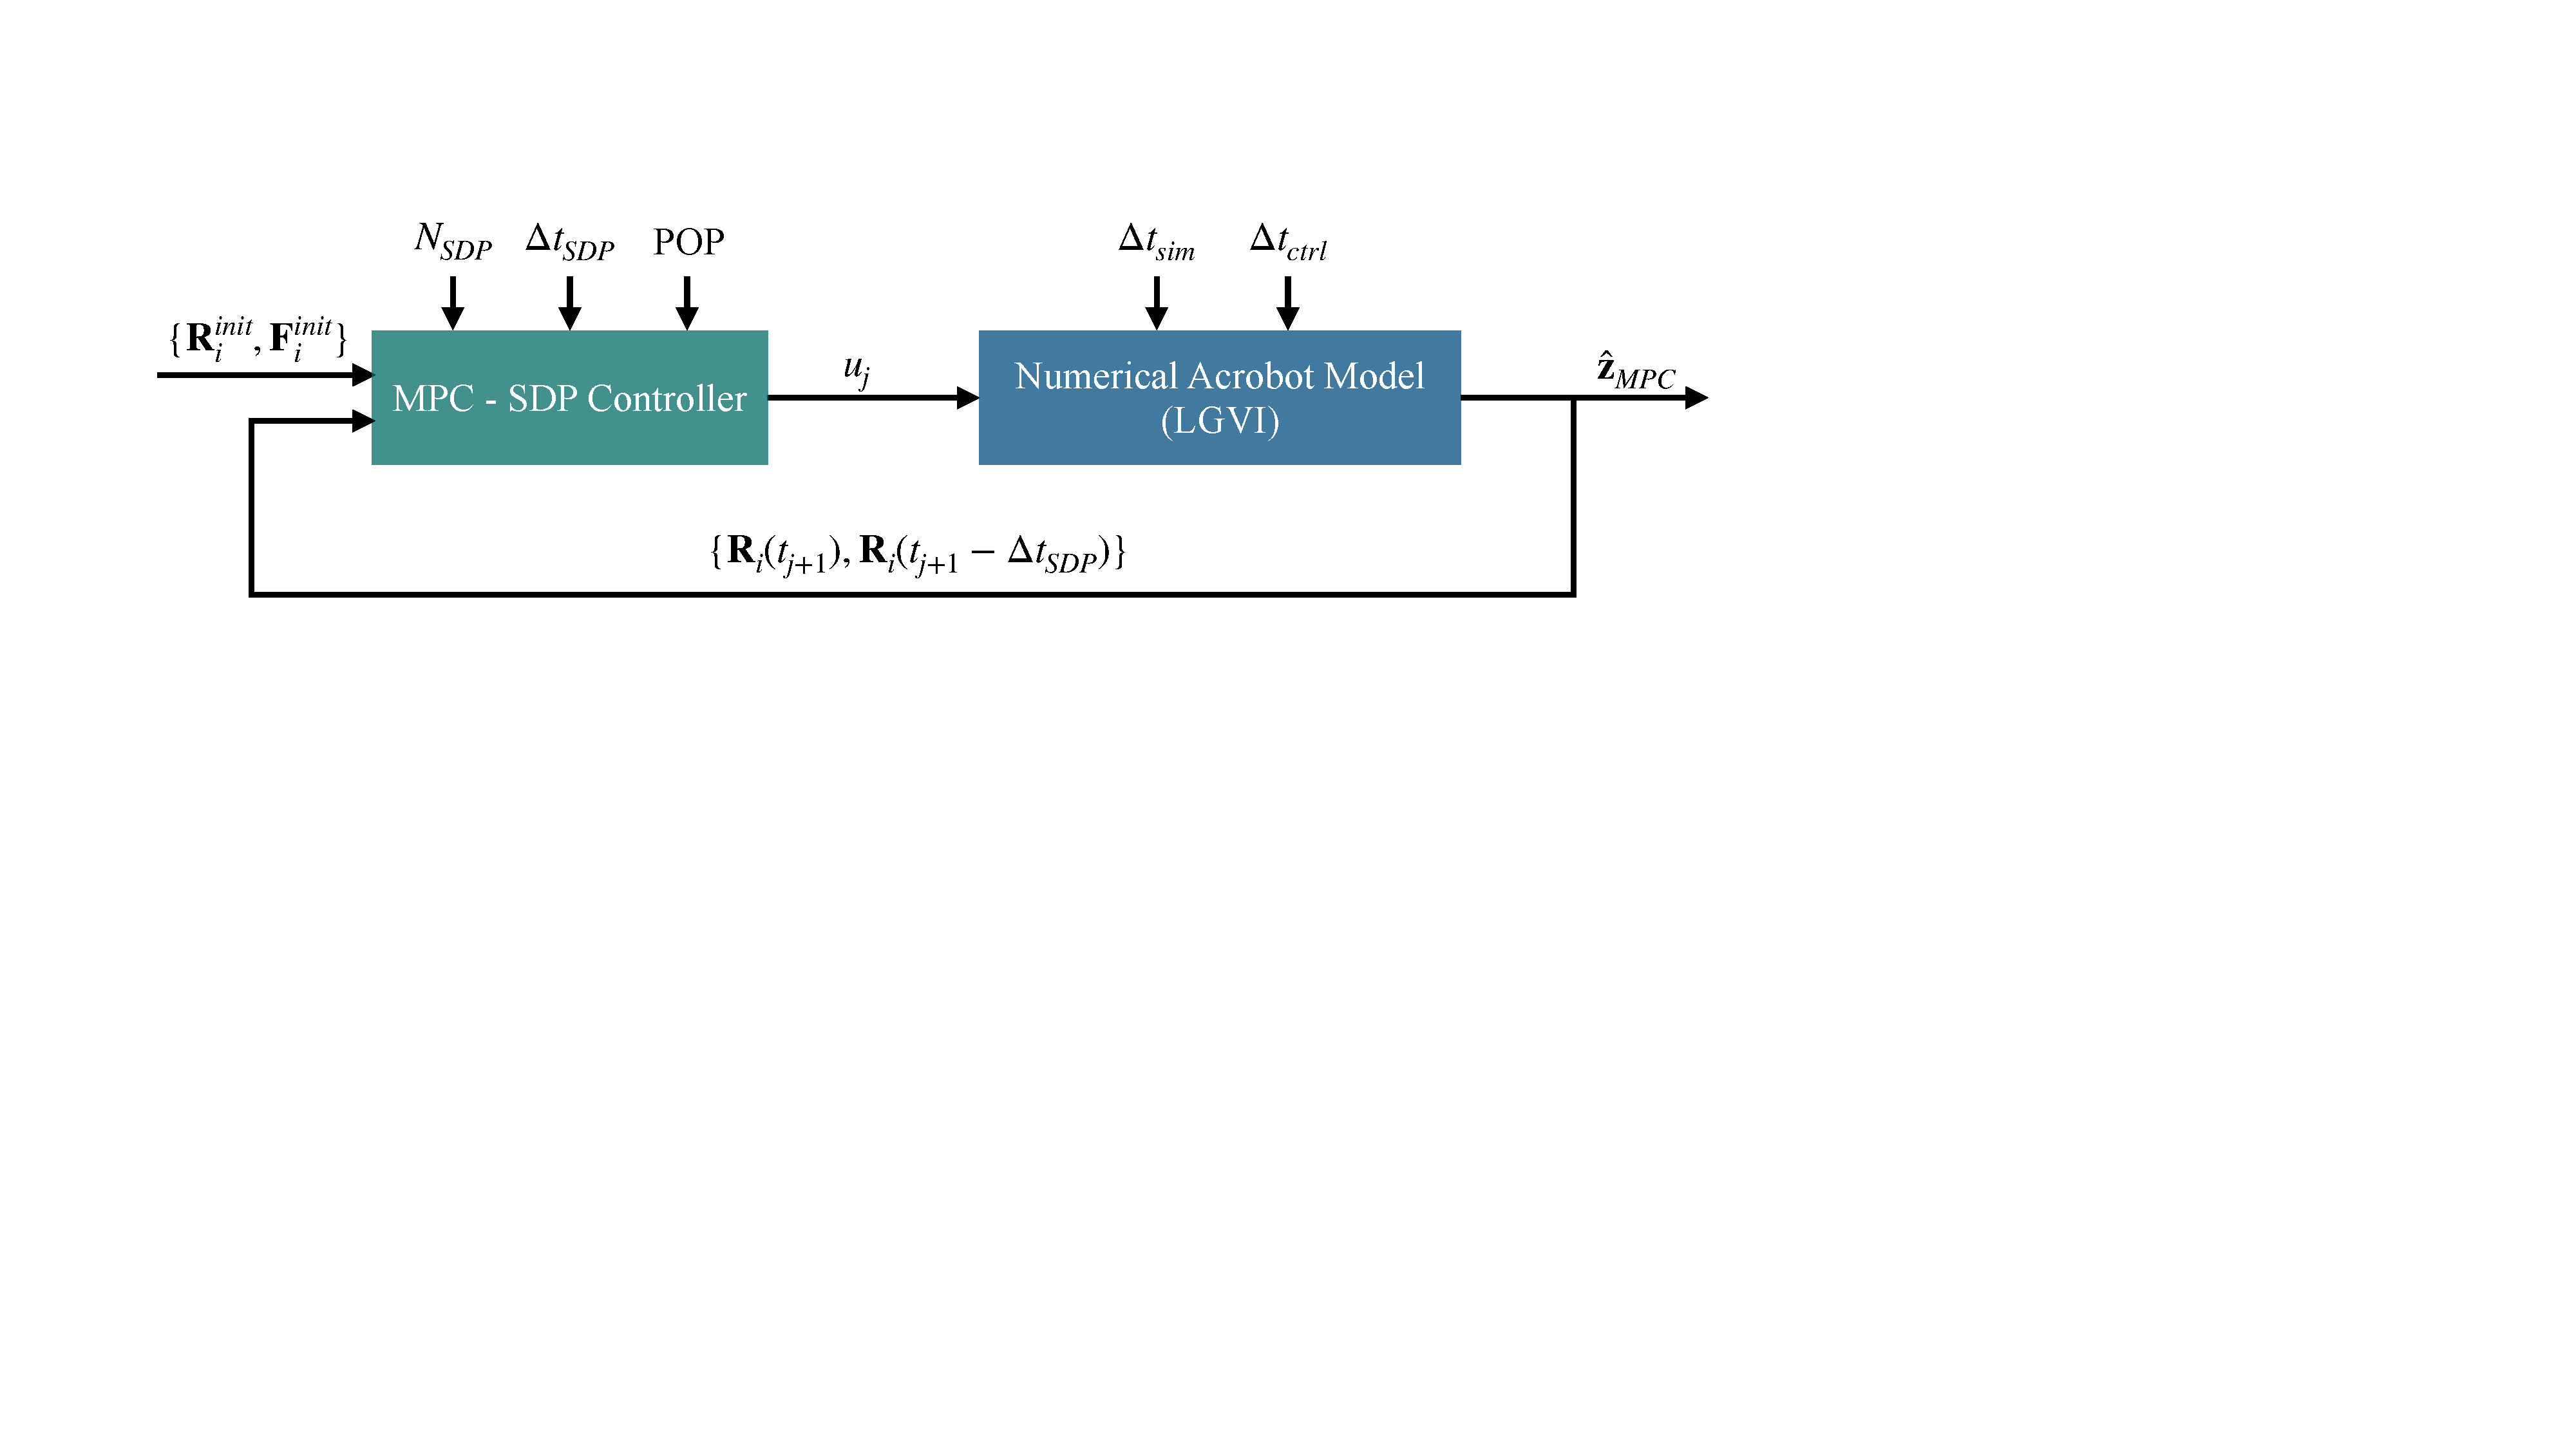
\includegraphics[width=\textwidth]{pics/Optimization/Acrobot/MPC_SDP_Loop.pdf}
    \caption{SDP-based model predictive control loop for the reduced Acrobot.}
    \label{fig:acrobot_sdp_mpc_loop}
\end{figure}

\paragraph{Receding-horizon}
In the following, \(j\in\mathbb{N}_0\) denotes the MPC iteration.
Therefore, the corresponding simulation time is
\begin{align}
t_j=j\Delta t_{\mathrm{ctrl}} 
\end{align}
In addition, \(k\mid j\) is the SDP prediction node \(k\)
of the problem solved at MPC iteration \(j\).
At every iteration, the second-order sparse Moment-SOS relaxation and
clique construction introduced in
Section~\ref{sec:trajectory_optimization_via_sdp_relaxation} are used.
Only the initial rotation data \(\bm{R}_{i,1\mid j}\), \(\bm{F}_{i,0\mid j}\), and
\(\bm{R}_{i,0\mid j}\) are updated from the simulated state, while the dynamics,
cost function, bounds, prediction horizon, and desired state remain unchanged.

For any two consecutive prediction nodes, the relative rotation satisfies
\begin{equation}
    \bm{F}_{i,k\mid j}
    =
    \bm{R}_{i,k\mid j}^{\top}\bm{R}_{i,k+1\mid j},
    \qquad
    \bm{R}_{i,k+1\mid j}
    =
    \bm{R}_{i,k\mid j}\bm{F}_{i,k\mid j}.
    \label{eq:acrobot_relative_rotation_general}
\end{equation}
At the boundary of each newly solved SDP problem, node \(k=1\) represents the
current simulated attitude at \(t_j\), whereas node \(k=0\) represents the
required history state one SDP interval earlier. Therefore, with
\(h=\Delta t_{\mathrm{SDP}}\), the updated boundary data are
\begin{equation}
\begin{aligned}
\bm{R}_{i,1\mid j}
&=\bm{R}_i(t_j),\\
\bm{F}_{i,0\mid j}
&=\bm{R}_i(t_j-\Delta t_{\mathrm{SDP}})^{\top}\bm{R}_i(t_j),\\
\bm{R}_{i,0\mid j}
&=\bm{R}_{i,1\mid j}\bm{F}_{i,0\mid j}^{\top},
\end{aligned}
\label{eq:acrobot_mpc_boundary_data}
\end{equation}
for links $i=1,2$.
The reconstruction \(\bm{F}_{i,0\mid j}=\bm{R}_i(t_j-\Delta t_{\mathrm{SDP}})^{\top}\bm{R}_i(t_j)\) ensures that the 
incoming relative rotation always spans exactly one SDP interval 
\(\Delta t_{\mathrm{SDP}}\). This is
important when the control interval \(\Delta t_{\mathrm{ctrl}}\) or the
simulation interval \(\Delta t_{\mathrm{sim}}\) differs from \(\Delta t_{\mathrm{SDP}}\).
However, during the first MPC iterations, the simulated state does not yet contain a full history
of past rotations for $\Delta t_{\mathrm{SDP}} > t_j$. Therefore, 
missing prehistory is completed using \(\bm{F}_i^{\mathrm{init}}=\bm{I}\),
simulating a stationary start.
\begin{align*}
\bm{R}_i(t)=\bm{R}_i(0)
\quad &\text{for } t<0, \\
\qquad
\bm{F}_{i,0\mid j}
=
\bm{R}_i(0)^\top \bm{R}_i(t_j)
\quad &\text{for }
0<t_j<\Delta t_{\mathrm{SDP}}.
\label{eq:initial_rotation_history}
\end{align*}

\paragraph{Control application}
After updating the boundary data at iteration \(j\), the reduced Acrobot POP
of Section~\ref{sec:trajectory_optimization_via_sdp_relaxation} is converted
into a second-order sparse SDP using SPOT and solved with MOSEK. Ordered
extraction of the degree-one moments provides the normalized first control
\(\bar u_{1\mid j}^{\star}\) from the solution vector 
\[\{\bar u_{1\mid j}^{\star}, \bar u_{2\mid j}^{\star},\dots, \bar u_{N_{\mathrm{SDP}}-1\mid j}^{\star}\}.\] The corresponding physical torque is
\begin{equation}
    u_j
    =
    u_{\max}\bar u_{1\mid j}^{\star}.
    \label{eq:acrobot_mpc_applied_control}
\end{equation}
Then, this first control $u_j$ is applied to the numerical Acrobot simulation 
of Section~\ref{subsec:evaluation_acrobot}, while the
remaining predicted control sequence is discarded. The control input
\(u_j\) is kept constant over the control interval 
$t_{j+1}=t_j+\Delta t_{\mathrm{ctrl}}$.
During this interval, the Acrobot is simulated using the reduced LGVI of
Section~\ref{subsection:discrete_Acrobot}. The simulated
trajectory at $j+1$ is then stored inside $\widehat{\bm{z}}_{\mathrm{MPC},j+1}$.
The resulting rotations and
rotation-steps are then used to construct the initial data for
the next SDP problem as described above. 

After the simulation interval, the rotation error \(e_{R,j}\) and the
relative-step rotation error \(e_{F,j}\) are evaluated. The latter is the
step-angle error calculated from the last fine simulation step and is measured
in degrees or radians, rather than degrees per second. The Acrobot is declared
stabilized if
\begin{equation}
    e_{R,j}\leq\varepsilon_R,
    \qquad
    e_{F,j}\leq\varepsilon_F
    \label{eq:acrobot_mpc_stabilization_condition}
\end{equation}
holds for \(n_{\mathrm{stable}}\) consecutive MPC updates. In this case, the
MPC loop terminates and the full simulated trajectory is 
saved inside $\widehat{\bm{z}}_{\mathrm{MPC},j+1}$. 
Otherwise, \(j\) is increased by one by the 
MPC-SDP controller, the initial data
is updated from the new simulated state, and the SDP is solved again. If the
SDP is infeasible or no finite first control can be extracted, the loop
terminates before another simulation interval.

\paragraph{Prediction horizon}
In summary, the MPC implementation uses
\begin{equation}
    \Delta t_{\mathrm{SDP}},
    \qquad
    \Delta t_{\mathrm{sim}},
    \qquad
    n_{\mathrm{sim}}
    =\frac{\Delta t_{\mathrm{ctrl}}}{\Delta t_{\mathrm{sim}}} \in \mathbb{N},
    \qquad
    T_{\mathrm{pred}}=(N_{\mathrm{SDP}}-1)\Delta t_{\mathrm{SDP}}.
    \label{eq:acrobot_mpc_time_scales}
\end{equation}
Here, \(\Delta t_{\mathrm{SDP}}\) is the discretization interval of the SDP prediction
model, \(\Delta t_{\mathrm{sim}}\) is the fine LGVI simulation step, and
\(\Delta t_{\mathrm{ctrl}}\) is the control interval between two MPC updates.
Consequently, the numerical plant performs \(n_{\mathrm{sim}}\) LGVI steps
before the SDP is solved again. The intervals \(\Delta t_{\mathrm{SDP}}\) and
\(\Delta t_{\mathrm{ctrl}}\) can differ from each other. If the two intervals are equal,
$\Delta t_{\mathrm{SDP}} = \Delta t_{\mathrm{ctrl}}$, one MPC
update corresponds to one predicted SDP interval.

Since node \(k=0\) contains the history state and node \(k=1\) the current
state, the \(N_{\mathrm{SDP}}-1\) future intervals give the prediction horizon
\(T_{\mathrm{pred}}=(N_{\mathrm{SDP}}-1)\Delta t_{\mathrm{SDP}}\).
Increasing \(N_{\mathrm{SDP}}\) 
provides a longer look-ahead for the swing-up but also increases the size
and solution time of the SDP. The complete decision logic of the SDP-based MPC loop is summarized in Figure~\ref{fig:acrobot_sdp_mpc_logic}.

\begin{figure}[!ht]
    \centering
    \resizebox{0.95\textwidth}{!}{%
        \begin{tikzpicture}[
    >=Stealth,
    font=\small,
    line/.style={draw, -{Stealth[length=2.2mm]}, line width=0.55pt},
    process/.style={
        draw,
        rectangle,
        align=center,
        minimum height=1.0cm,
        text width=4.6cm,
        inner xsep=3mm,
        inner ysep=2mm
    },
    wideprocess/.style={
        process,
        minimum height=1.15cm,
        text width=8.4cm
    },
    smallprocess/.style={
        process,
        minimum height=0.75cm,
        text width=4.2cm
    },
    decision/.style={
        draw,
        diamond,
        aspect=1.35,
        align=center,
        inner sep=1.5pt,
        text width=2.5cm
    },
    terminalbad/.style={
        process,
        draw=red,
        text width=3.7cm,
        minimum height=0.75cm,
        fill=red!3
    },
    terminalgood/.style={
        process,
        draw=green!65!black,
        text width=3.8cm,
        minimum height=0.75cm,
        fill=green!5
    }
]

\node[wideprocess] (update) at (4.25, -1.25)
    {Update SDP initial states\\[0.2em]
     \textcolor{red}{\eqref{eq:acrobot_mpc_boundary_data}}};

\node[draw, circle, minimum size=7mm, inner sep=0pt] (start) at ($(update.north)+(0,1.25cm)$) {};
\node[align=center, right=2mm of start] (initial) {$\bm{R}_i^{\mathrm{init}},\,\bm{F}_i^{\mathrm{init}}$};

\node[process, below left=1.05cm and 2.95cm of update.south] (solve)
    {Solve POP \textcolor{red}{\eqref{eq:controlled_acrobot_pop}} via SDP\\[0.2em]
     $\rightarrow$ extract $\bar u_{1\mid j}^{\star}$};

\node[terminalbad, below right=0.95cm and 0.15cm of solve.south east] (infeasible)
    {Terminate};

\node[smallprocess, below=1.95cm of solve, xshift=-1.2cm] (simulate)
    {Numerical simulation\\
     Acrobot LGVI \textcolor{red}{\eqref{eq:acrobot_full_del_shifted}}};

\node[smallprocess, below=0.8cm of simulate] (error)
    {Compute $e_{R,j+1},\,e_{\omega,j+1}$};

\node[decision, below right=0.9cm and 1.9cm of error.south] (terminal)
    {Check\\terminal\\condition\\
     \textcolor{red}{\eqref{eq:acrobot_mpc_stabilization_condition}}};

\node[terminalgood, below=0.9cm of terminal] (trajectory)
    {MPC trajectory $\bm{\hat{z}}_{\mathrm{A},\mathrm{mpc}}$};

\draw[line] (start) -- (update);

\draw[line]
    (update.west) -- (solve.north |- update.west) -- (solve.north);

\draw[line]
    (solve.south) -- ++(0,-0.55cm)
    -| node[pos=0.72, right, align=left] {Apply control $u_j$\\[-0.1em]
        \textcolor{red}{\eqref{eq:acrobot_mpc_applied_control}}}
    (simulate.north);

\draw[line]
    (solve.east) -- node[above] {infeasible} (infeasible.north |- solve.east)
    -- (infeasible.north);

\draw[line]
    (simulate.south) -- node[right] {$\bm{\hat{z}}_{\mathrm{A},\mathrm{MPC},j+1}$} (error.north);

\draw[line] (error.south) |- (terminal.west);

\draw[line]
    (terminal.south) -- node[right] {Yes} (trajectory.north);

\draw[line]
    (terminal.east) .. controls +(3.7cm,0.8cm) and +(1.6cm,-1.6cm) ..
    node[pos=0.31, anchor=west, xshift=10pt, fill=white, inner sep=1pt] {No: $j \leftarrow j+1$}
    (update.south east);

\end{tikzpicture}
%
    }
    \caption{Decision logic of the SDP-based model predictive control loop for the reduced Acrobot.}
    \label{fig:acrobot_sdp_mpc_logic}
\end{figure}
